\documentclass{beamer}
\usetheme{Frankfurt}
\usepackage[utf8]{inputenc}

\usepackage{algorithmic}
\usepackage{algorithm}
{\renewcommand{\bibname}{References}}  
\usepackage[backend=bibtex,style=numeric]{biblatex}  %backend=biber is 'better
\renewcommand{\algorithmicrequire}{\textbf{Input:}}
\renewcommand{\algorithmicensure}{\textbf{Output:}}

\usepackage{amssymb}
\usepackage{amsfonts}
\usepackage{amsmath}
\newcommand{\argmin}{\mathop{\mathrm{arg\,min}}\limits}
\newcommand{\argmax}{\mathop{\mathrm{arg\,max}}\limits}
\newcommand{\mymin}{\mathop{\mathrm{min}}\limits}
\addbibresource{references.bib}  

\graphicspath{ {./images/} }

\usepackage{xspace}

\usepackage{multirow}
\usepackage{booktabs}

\title[A GRASP metaheuristic for a TDP]
{A GRASP metaheuristic for a territorial design problem in financial institutions}
\author{Eduardo Salazar Treviño, Roger Z. Ríos Mercado, Diana L. Huerta Muñoz}
\institute[]{
    Department of Mechanical and Electrical Engineering \\
    Universidad Autónoma de Nuevo León \\
    San Nicolás de los Garza, N.L.
}
\date[X CSMIO]{
    XI Congreso de la Sociedad Mexicana de Investigación de Operaciones \\ 
    October 19th, 2023
}
\begin{document}

\begin{frame}
    \titlepage
\end{frame}

\begin{frame}{Outline}
    \tableofcontents
\end{frame}

\section{Problem statement and motivation}

\begin{frame}{Territorial Design Problem}
    \framesubtitle{Problem formulation}
    According to \cite{cor2009}, a classic Territorial Design Problem, also known as a Districting Problem, organizes and partitionates a given set $B$ of small geographical units, or \textit{basic units} (BUs) and a set $S$ of centers into $p$ larger geographical clusters known as territories or districts, according to spatial constraints such as compactness, contiguity; planning constraints in order to balance the magnitude of activities performed across all territories, such as sales, total workload, etc. In order to get compact territories, a dispersion measure  based on the objective function of several classic location problems, such as the p-center problem or the p-median problem must be considered.
\end{frame}

\begin{frame}{Microfinancial institutions and applications}
    \framesubtitle{Problem formulation}
    The model described in this work is motivated by a previous model described in \cite{jimo2020} which presents an application of a TDP to a real life microfinancial institution. Microfinance institutions (MFIs) are important to reduce income inequality and poverty. They offer credit and other financial products to markets that are normally rejected by commercial banks as they represent high-risk with low-profit.
\end{frame}

\begin{frame}{Microfinancial institutions' special requirements}
    \framesubtitle{Problem formulation}
    In this context, the TDP first identifies which potential locations will house a branch office of the institution. Given that these branches are set up within pre-existing business establishments, it's crucial to ensure a balanced distribution of these centers across every line of business of the host location. Beyond evenly spreading activity metrics like total loan amounts, workload, and client count, it's also essential to balance the risk associated with granted loans due to their inherent volatility across all territories. The objective function minimizes the sum of distances from BUs to their assigned institution's branches.
\end{frame}

\begin{frame}{Financial institution territory example}
    \framesubtitle{Instance example}
    \begin{figure}
        \centering
        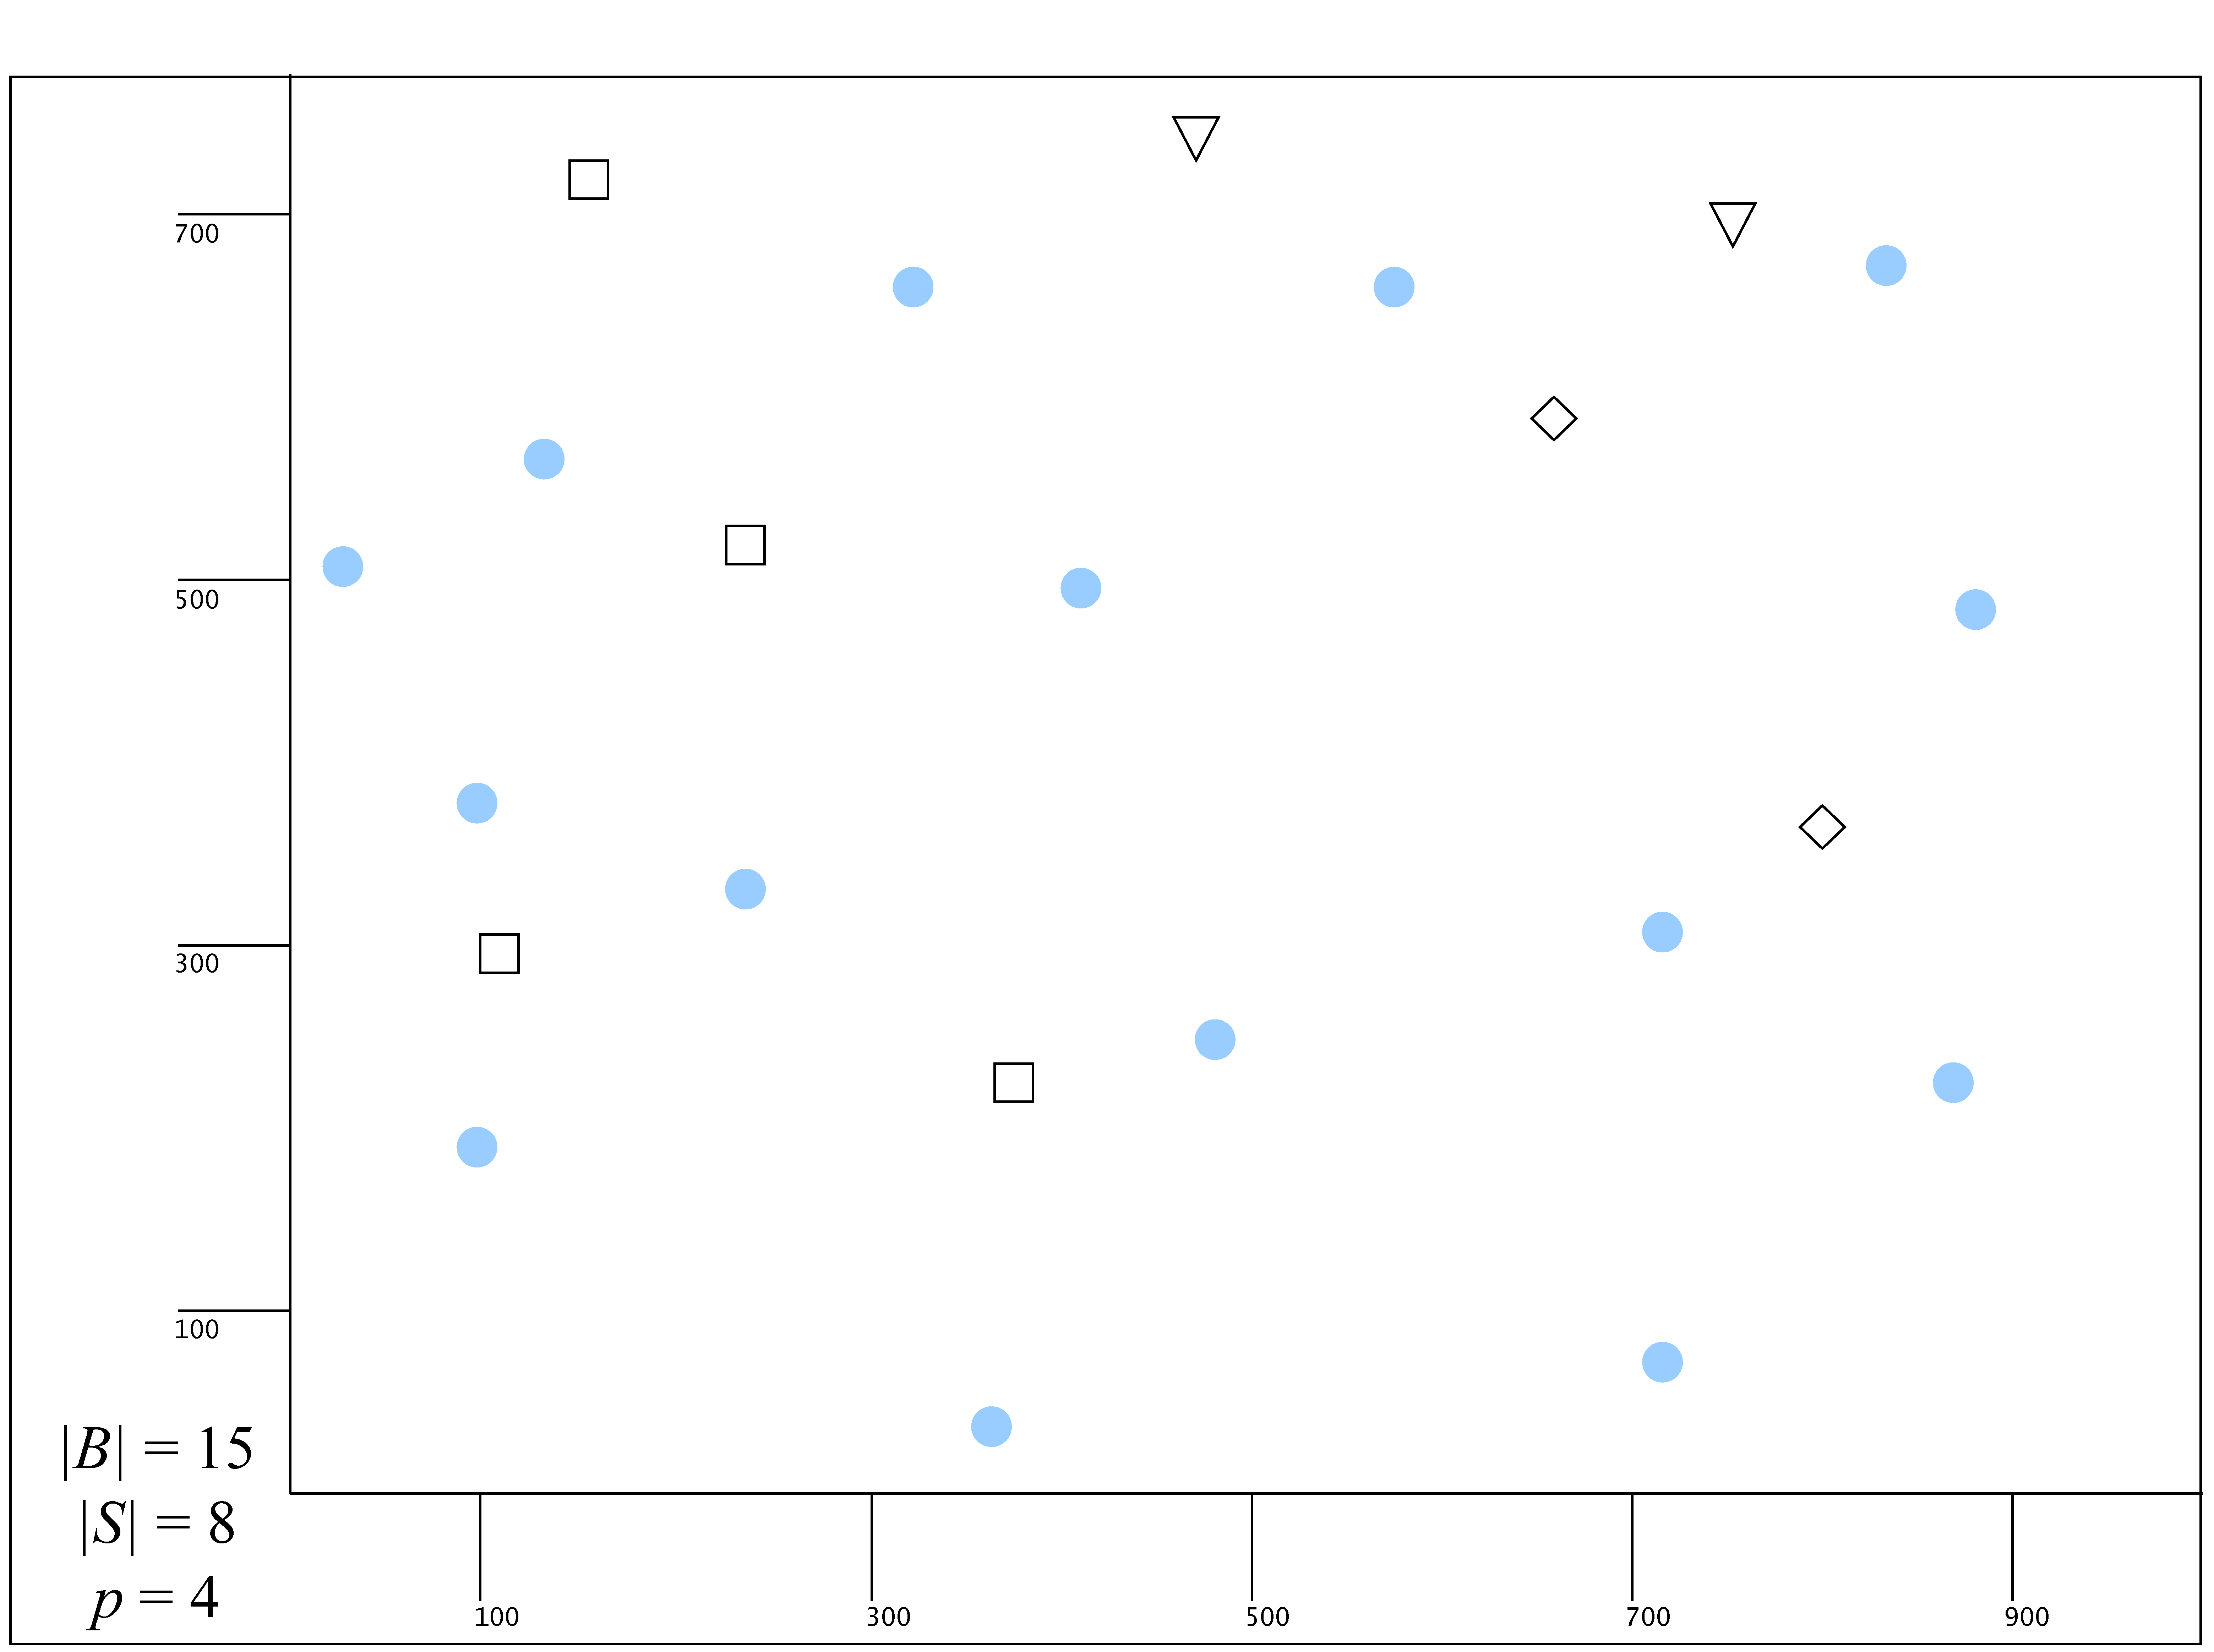
\includegraphics[scale=0.08]{instancia_dpi.pdf}
        \label{fig:instancia}
    \end{figure}
\end{frame}

\begin{frame}{Financial institution territory example}
    \framesubtitle{Feasible solution example}
    \begin{figure}
        \centering
        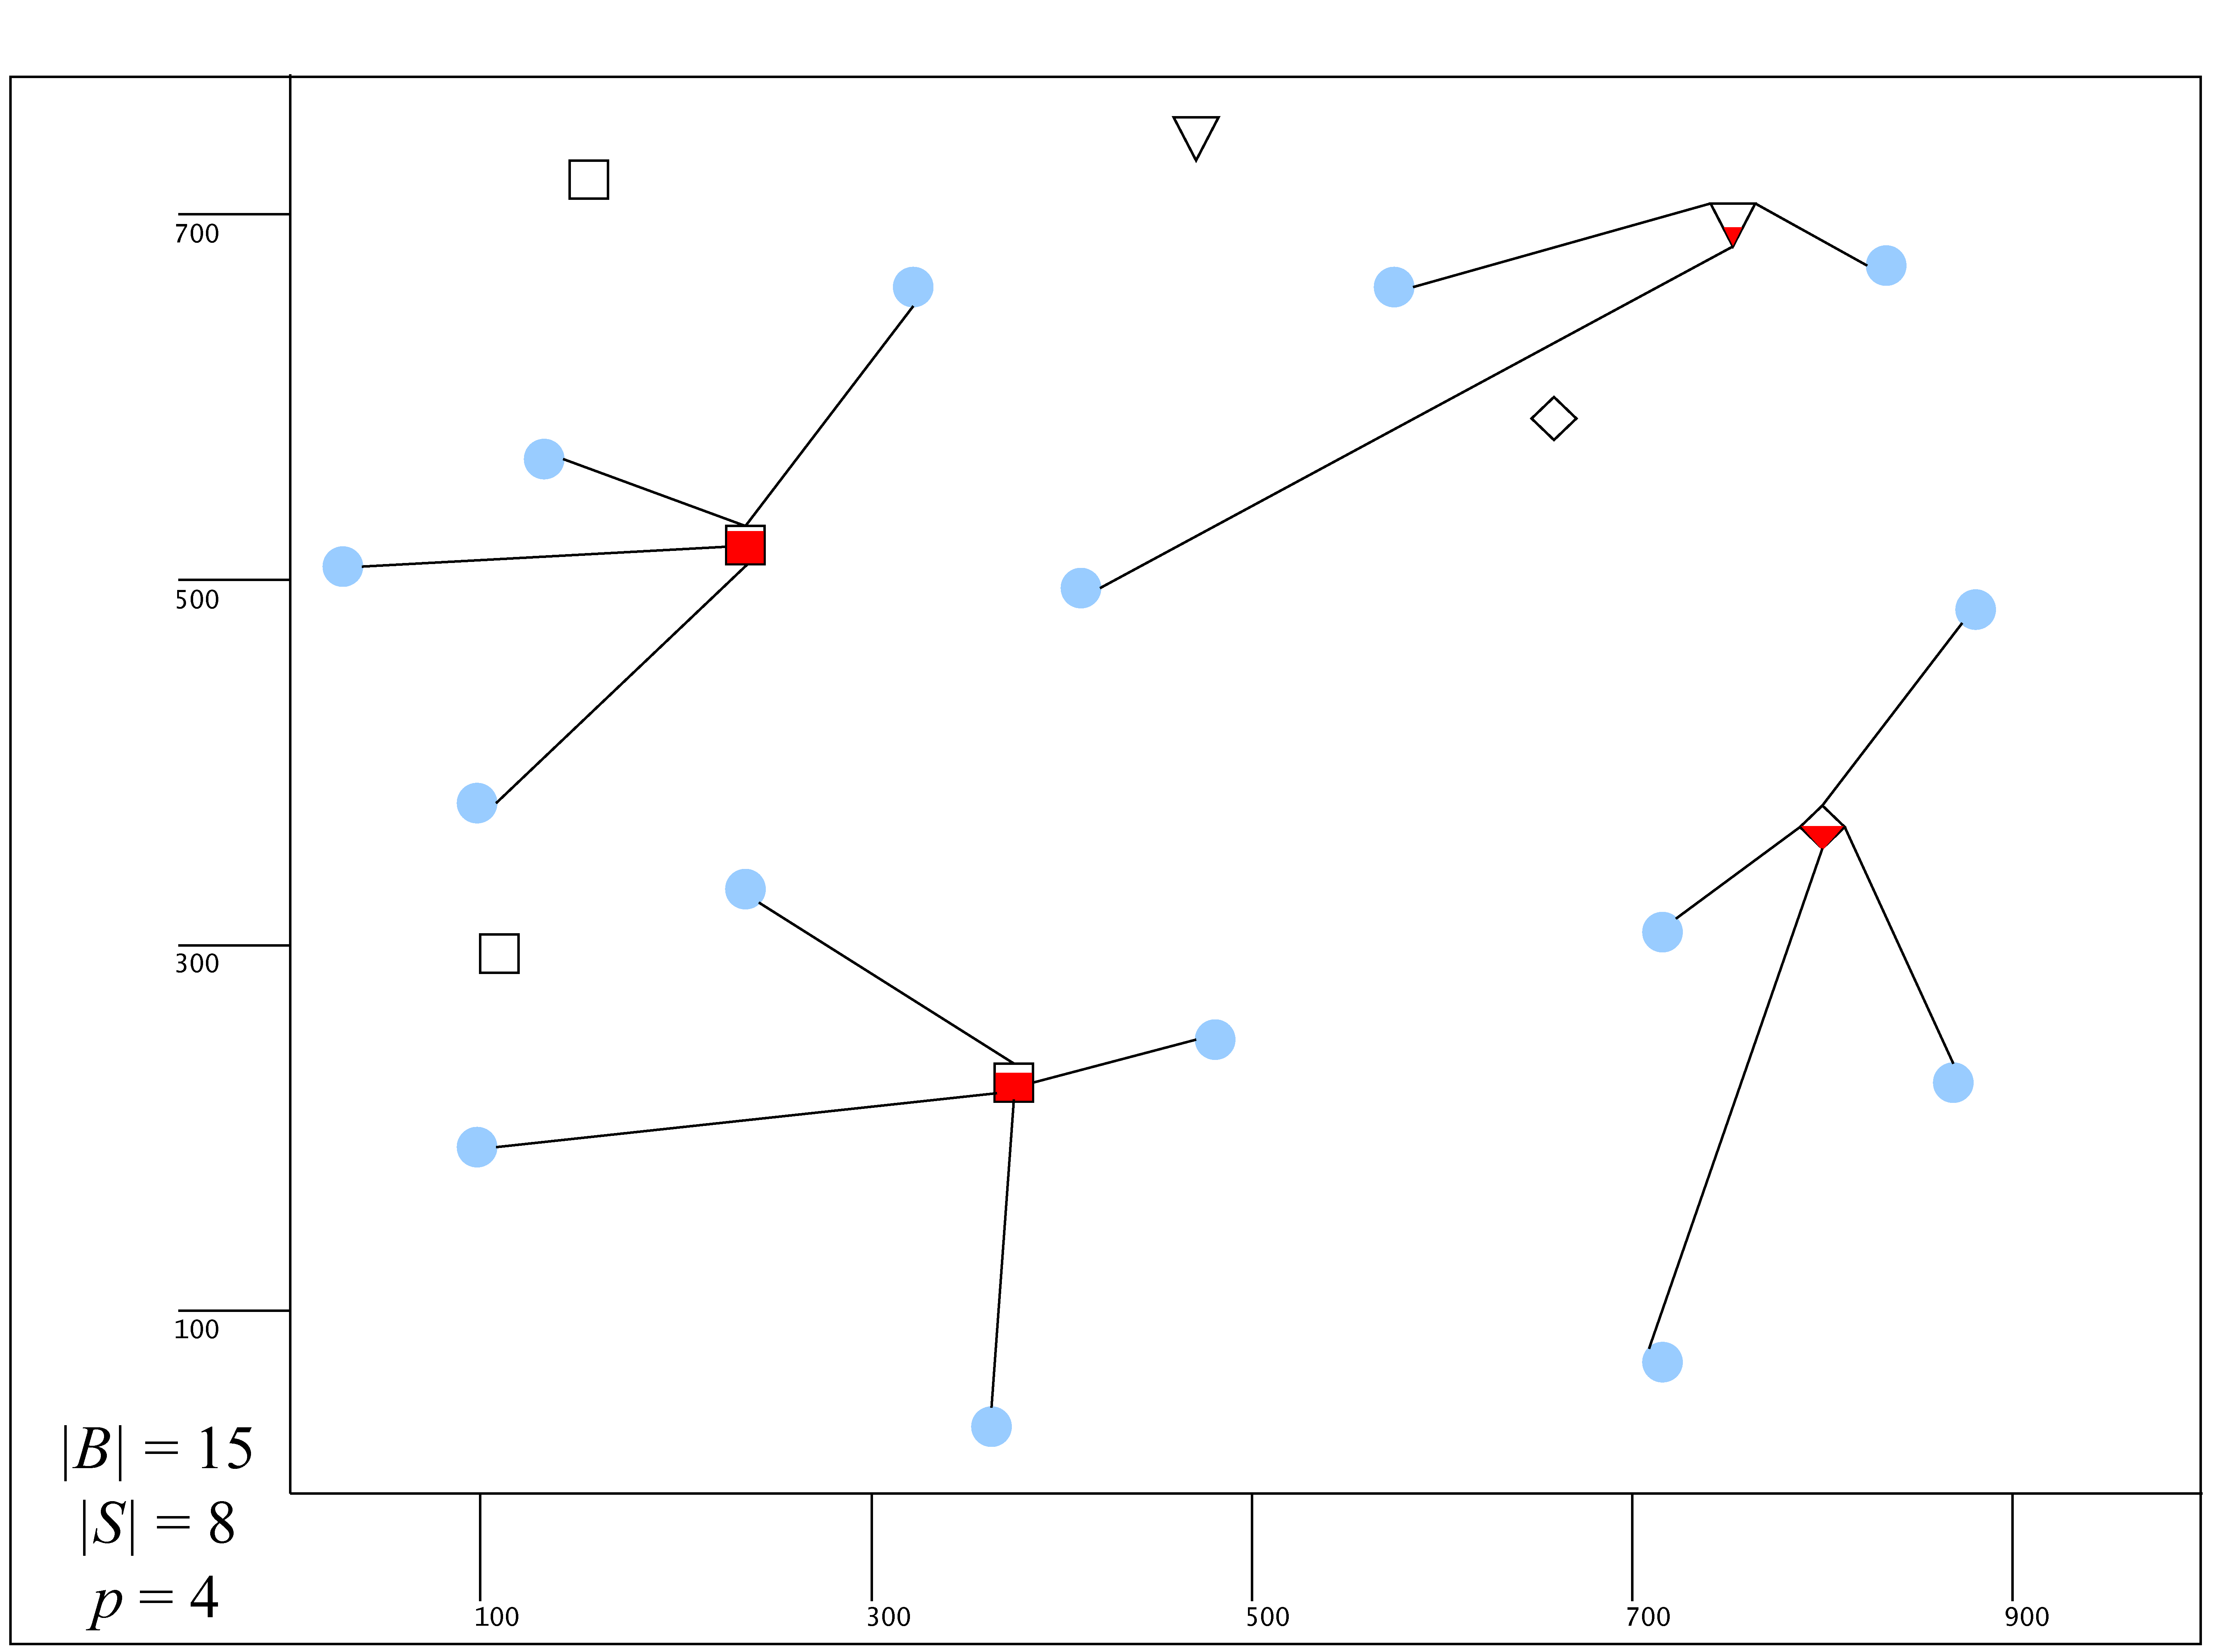
\includegraphics[scale=0.08]{solucion_buena_dpi.pdf}
        \label{fig:instancia}
    \end{figure}
\end{frame}

\begin{frame}{Financial institution territory example}
    \framesubtitle{Unfeasible solution example}
    \begin{figure}
        \centering
        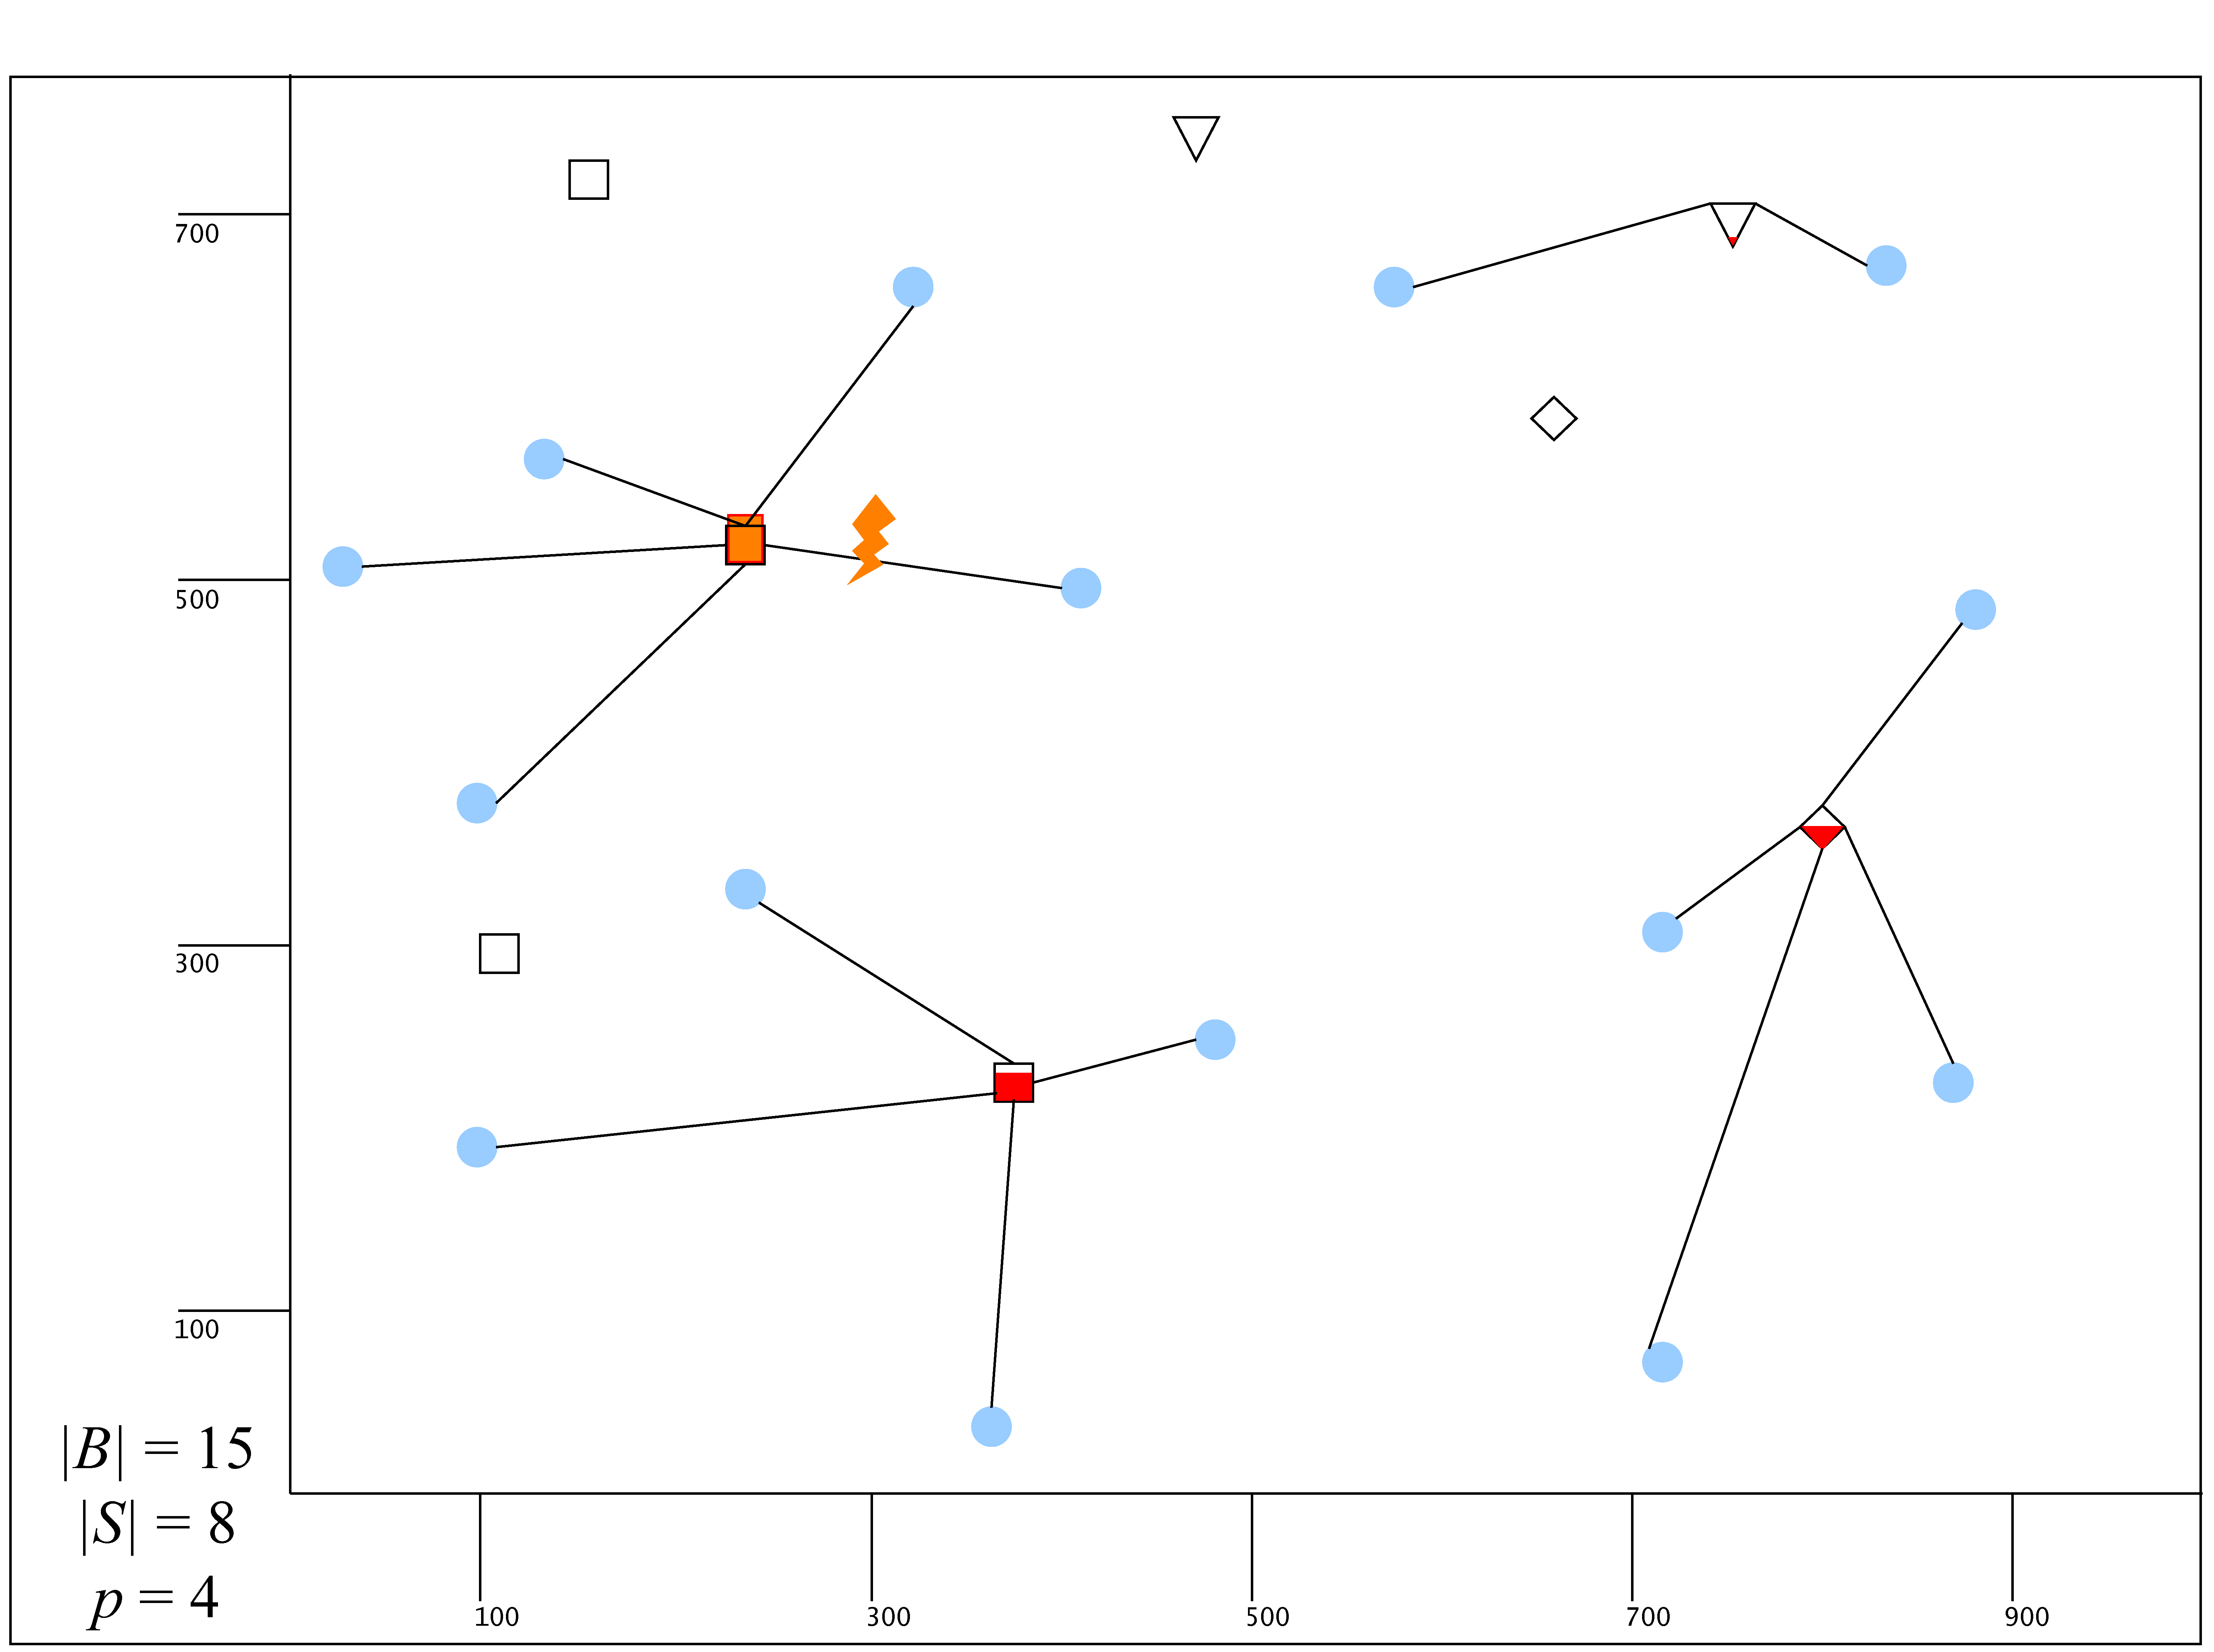
\includegraphics[scale=0.08]{inst_mala.pdf}
        \label{fig:instancia}
    \end{figure}
\end{frame}

\begin{frame}{Motivation and Purpose}
    Compared to the previous model, this model incorporates risk balancing as a constraint, while the former treats it as part of the objective function. Furthermore, the previous model was applied to an existing territorial design, so its objective function also included a term to retain as much of the original design as possible. This model does not consider contiguity as a constraint.
    \\
    This model can be likened to a vertex p-center problem with multiple capacity constraints. Considering that even the uncapacitated vertex p-center problem is NP-hard \cite{eswa2016}, our TDP is also NP-hard. This highlights the potential value of heuristic approaches for solving it.
\end{frame}

\begin{frame}{Combinatorial model}
    \framesubtitle{Problem formulation}
        Sets and parameters
        \begin{itemize}
            \item $S = \{1, 2, ..., s\}$, set of possible territory centers
            \item $B = \{1, 2, ..., b\}$, set of possible BUs
            \item $d_{ij}$, distance matrix between center $i$ and BU $j$, $i \in S, j \in B$
            \item $M = \{1,2, ..., m\}$, set of activity measures
            \item $\mu_m^i$,  target of activity $m, m \in M$ measure at center $i, i \in S$
            \item $v_m^j$, measure of activity $m$ at BU $j, j\in B$
            \item $t_m$, tolerance of activity $m$ measure
            \item $R_j$, risk value at BU $j$
            \item $\beta_i$, risk threshold at center $i \in S$
            \item $S_k = \{1,2,...,s\}$, 1 if $s \in S$ is of type $k$, 0 otherwise, $k \in \{1\ldots 5\}$
            \item $L_k, U_k$, lower and upper bounds of centers to be used for each $S_k$
            \item $p$, number of centers to be used
        \end{itemize}
        
\end{frame}

\begin{frame}{Combinatorial model}
    \framesubtitle{Problem formulation}
        Decision Variables 
        \begin{itemize}
            \item \small $Y_i$, 1 if the center $i$ is used; otherwise 0.
            \item \small $X_{ij}$, 1 if the BU $j$ is assigned to center $i$; otherwise 0.
        \end{itemize}
\end{frame}

        


\begin{frame}{Mathematical programming}
    \framesubtitle{Formulation}
    Objective Function:
    \begin{equation}
        \mathbf{min}\sum_{i \in S, j \in B}{X_{ij} D_{ij}}
    \end{equation}{}
    Subject to:
    \begin{equation}
       \sum_{i \in S} X_{ij} = 1, \quad \forall j \in B
    \end{equation}{}
    \centering \small Single assignment of a BU $j$ to a center $i$
    \begin{equation}
        X_{ij} \le Y_i, \quad \forall i \in S, \quad j \in B
    \end{equation}{}
    Can only assign BUs to centers that are open
    \begin{equation}
        Y_i\mu_m^i(1-t^m) \le \sum_{j\in B}X_{ij}v_j^m \le Y_i\mu_m^i(1+t^m), \quad \forall i \in S
    \end{equation}{}
    Activity measures for each territory must be within a tolerance range
\end{frame}

\begin{frame}{Mathematical programming}
    \framesubtitle{Formulation}
    \begin{equation}
        l_k \le \sum_{i \in S_k} Y_i \le u_k, \quad k \in \{1 \ldots 5\}
    \end{equation}{}
    The selected centers' types must respect the lower and upper bound for each type
    \begin{equation}
        \sum_{i \in S} Y_i = P
    \end{equation}{}
    The number of centers to be opened must be equal to $P$
    \begin{equation}
        \sum_{j \in B}X_{ij}R_j \le \beta_i, \quad \forall i \in S
    \end{equation}{}
    The risk measure of each territory must not surpass the risk threshold
\end{frame}

\section{Proposed heuristic}

\begin{frame}{Proposed heuristic}
    \begin{columns}
        \column{0.65\textwidth}
        \begin{algorithmic}[1]
        
        \REQUIRE $p, \alpha_l, \alpha_a, i_{max}$, Instance
        \ENSURE $X,Y$ = binary decision variables
        
        \STATE $A^* \gets \emptyset$
        \STATE $f^* \gets \infty$
        \WHILE {$i_{max} > 0$}
            \STATE $X, Y \gets$ Construct($\alpha_l, \alpha_a, p$, Instance)
            \STATE $X, Y \gets$ LocalSearch($X, Y,$ Instance)
            \STATE $A \gets (X, Y)$
            \IF {$f(A) < f^*$}
                \STATE $f^* \gets f(A)$
                \STATE $A^* \gets A$ 
            \ENDIF
            \STATE $i_{max} \gets i_{max} - 1$
        \ENDWHILE
        \RETURN $A^*$
        
        \end{algorithmic}
        
        \column{0.35\textwidth}
        A metaheuristic framework with a Greedy Randomized Adaptive Search Procedure (GRASP) using a value-based restricted candidate list (RCL).
        Parameters:
        \begin{itemize}
            \item $\alpha_l, \alpha_a$: Threshold quality parameters
            \item $i_{max}$: Number of iterations
        \end{itemize}
    \end{columns}
\end{frame}

\begin{frame}{Construction phase}
    The constructive heuristic used in this work consists of two phases: Location and Allocation. \\
    In the Location phase, we must first determine which $p$ centers are to be used out of all the available possible locations. This phase returns the decision variable vector $Y$. \\
    The Allocation phase will allocate all the BUs to a corresponding center. This phase will return the decision variable matrix $X$. \\
\end{frame}

\begin{frame}{Construction phase}
    \framesubtitle{Location heuristics}
    \begin{itemize}
        \item $p$-dispersion problem: Select the $p$-most disperse centers out of $S$ while respecting $L_k$ and $U_k$ with the best current polynomial-time heuristic according to \cite{ravi_heuristic_1994}
        \item Relaxation of integer constraints: Solve the exact formulation, relax integer bounds of $X$, thus providing $Y$ with integer values.
    \end{itemize}
\end{frame}

\begin{frame}{Construction phase}
    \framesubtitle{PDISP\_SIMPLE}
    \scalebox{0.9}{
    \begin{minipage}{1.8\linewidth}
            \begin{algorithmic}[1]
            \REQUIRE distanceMatrix, $p$, totalNodes
            \ENSURE SolutionSet of nodes for p-dispersion problem
            \STATE Find the pair of nodes with the maximum distance in distanceMatrix
            \STATE Initialize SolutionSet with these two nodes
            \WHILE{$\lvert SolutionSet\rvert < p$}
                \FOR{node $\in$ totalNodes}
                    \IF{node $\notin$ SolutionSet}
                        \STATE Find the shortest distance from node to any node in SolutionSet
                        \STATE Store this shortest distance along with the node
                    \ENDIF
                \ENDFOR
                \STATE Select the node with the maximum shortest distance
                \STATE Add this node to SolutionSet
            \ENDWHILE
            \RETURN SolutionSet
        \end{algorithmic}
    \end{minipage}
    }
\end{frame}

\begin{frame}{Construction phase}
    \framesubtitle{$p$-dispersion problem}
    \scalebox{0.8}{
    \begin{minipage}{1.8\linewidth}
        \begin{algorithmic}[1]
        \REQUIRE $d$, $p$, $S_k$, $L_k$, $U_k$, $S$
        \ENSURE $Y$
        \STATE Compute distance matrices, $\forall k \in S_k$
        \FOR{$k \in S_k$}
            \STATE PDISP\_SIMPLE(distance matrix of $k$, $L_k$, $\lvert S_k \rvert)$
            \STATE Add to $Y$ the solution provided for each $k$
        \ENDFOR
        \WHILE{$\lvert Y \rvert < p$}
            \FOR{node in $S$}
                \IF{node $\notin Y$ }
                    \STATE Determine type of node in $S_k$
                    \STATE Check if $U_k$ for this node type is reached; if so, skip this node
                    \STATE Compute the minimum distance to the nodes in $Y$
                    \STATE Store this minimum distance with the node
                \ENDIF
            \ENDFOR
            \STATE Select the node with the maximum minimum distance
            \STATE Add this node to $Y$
        \ENDWHILE
        \RETURN $Y$
        \end{algorithmic}
    \end{minipage}
    }
\end{frame}


\begin{frame}{Construction phase}
    \framesubtitle{Allocation heuristics}
    Due to the constrained nature of the problem, the nearest assignment for each BU will not always be valid. Instead of selecting the minimal distances, we calculate the cost of opportunity for all BUs, prioritizing the assignments of those with the largest opportunity cost.
    \begin{itemize}
        \item Cost of opportunity.
        \item Cost of opportunity enhanced with data structures.
    \end{itemize}
    
\end{frame}

\begin{frame}{Cost of Opportunity}
    \framesubtitle{Explanation}
    Let us pick two arbitrary BUs, obtaining their nearest center:
    \begin{figure}
        \centering
        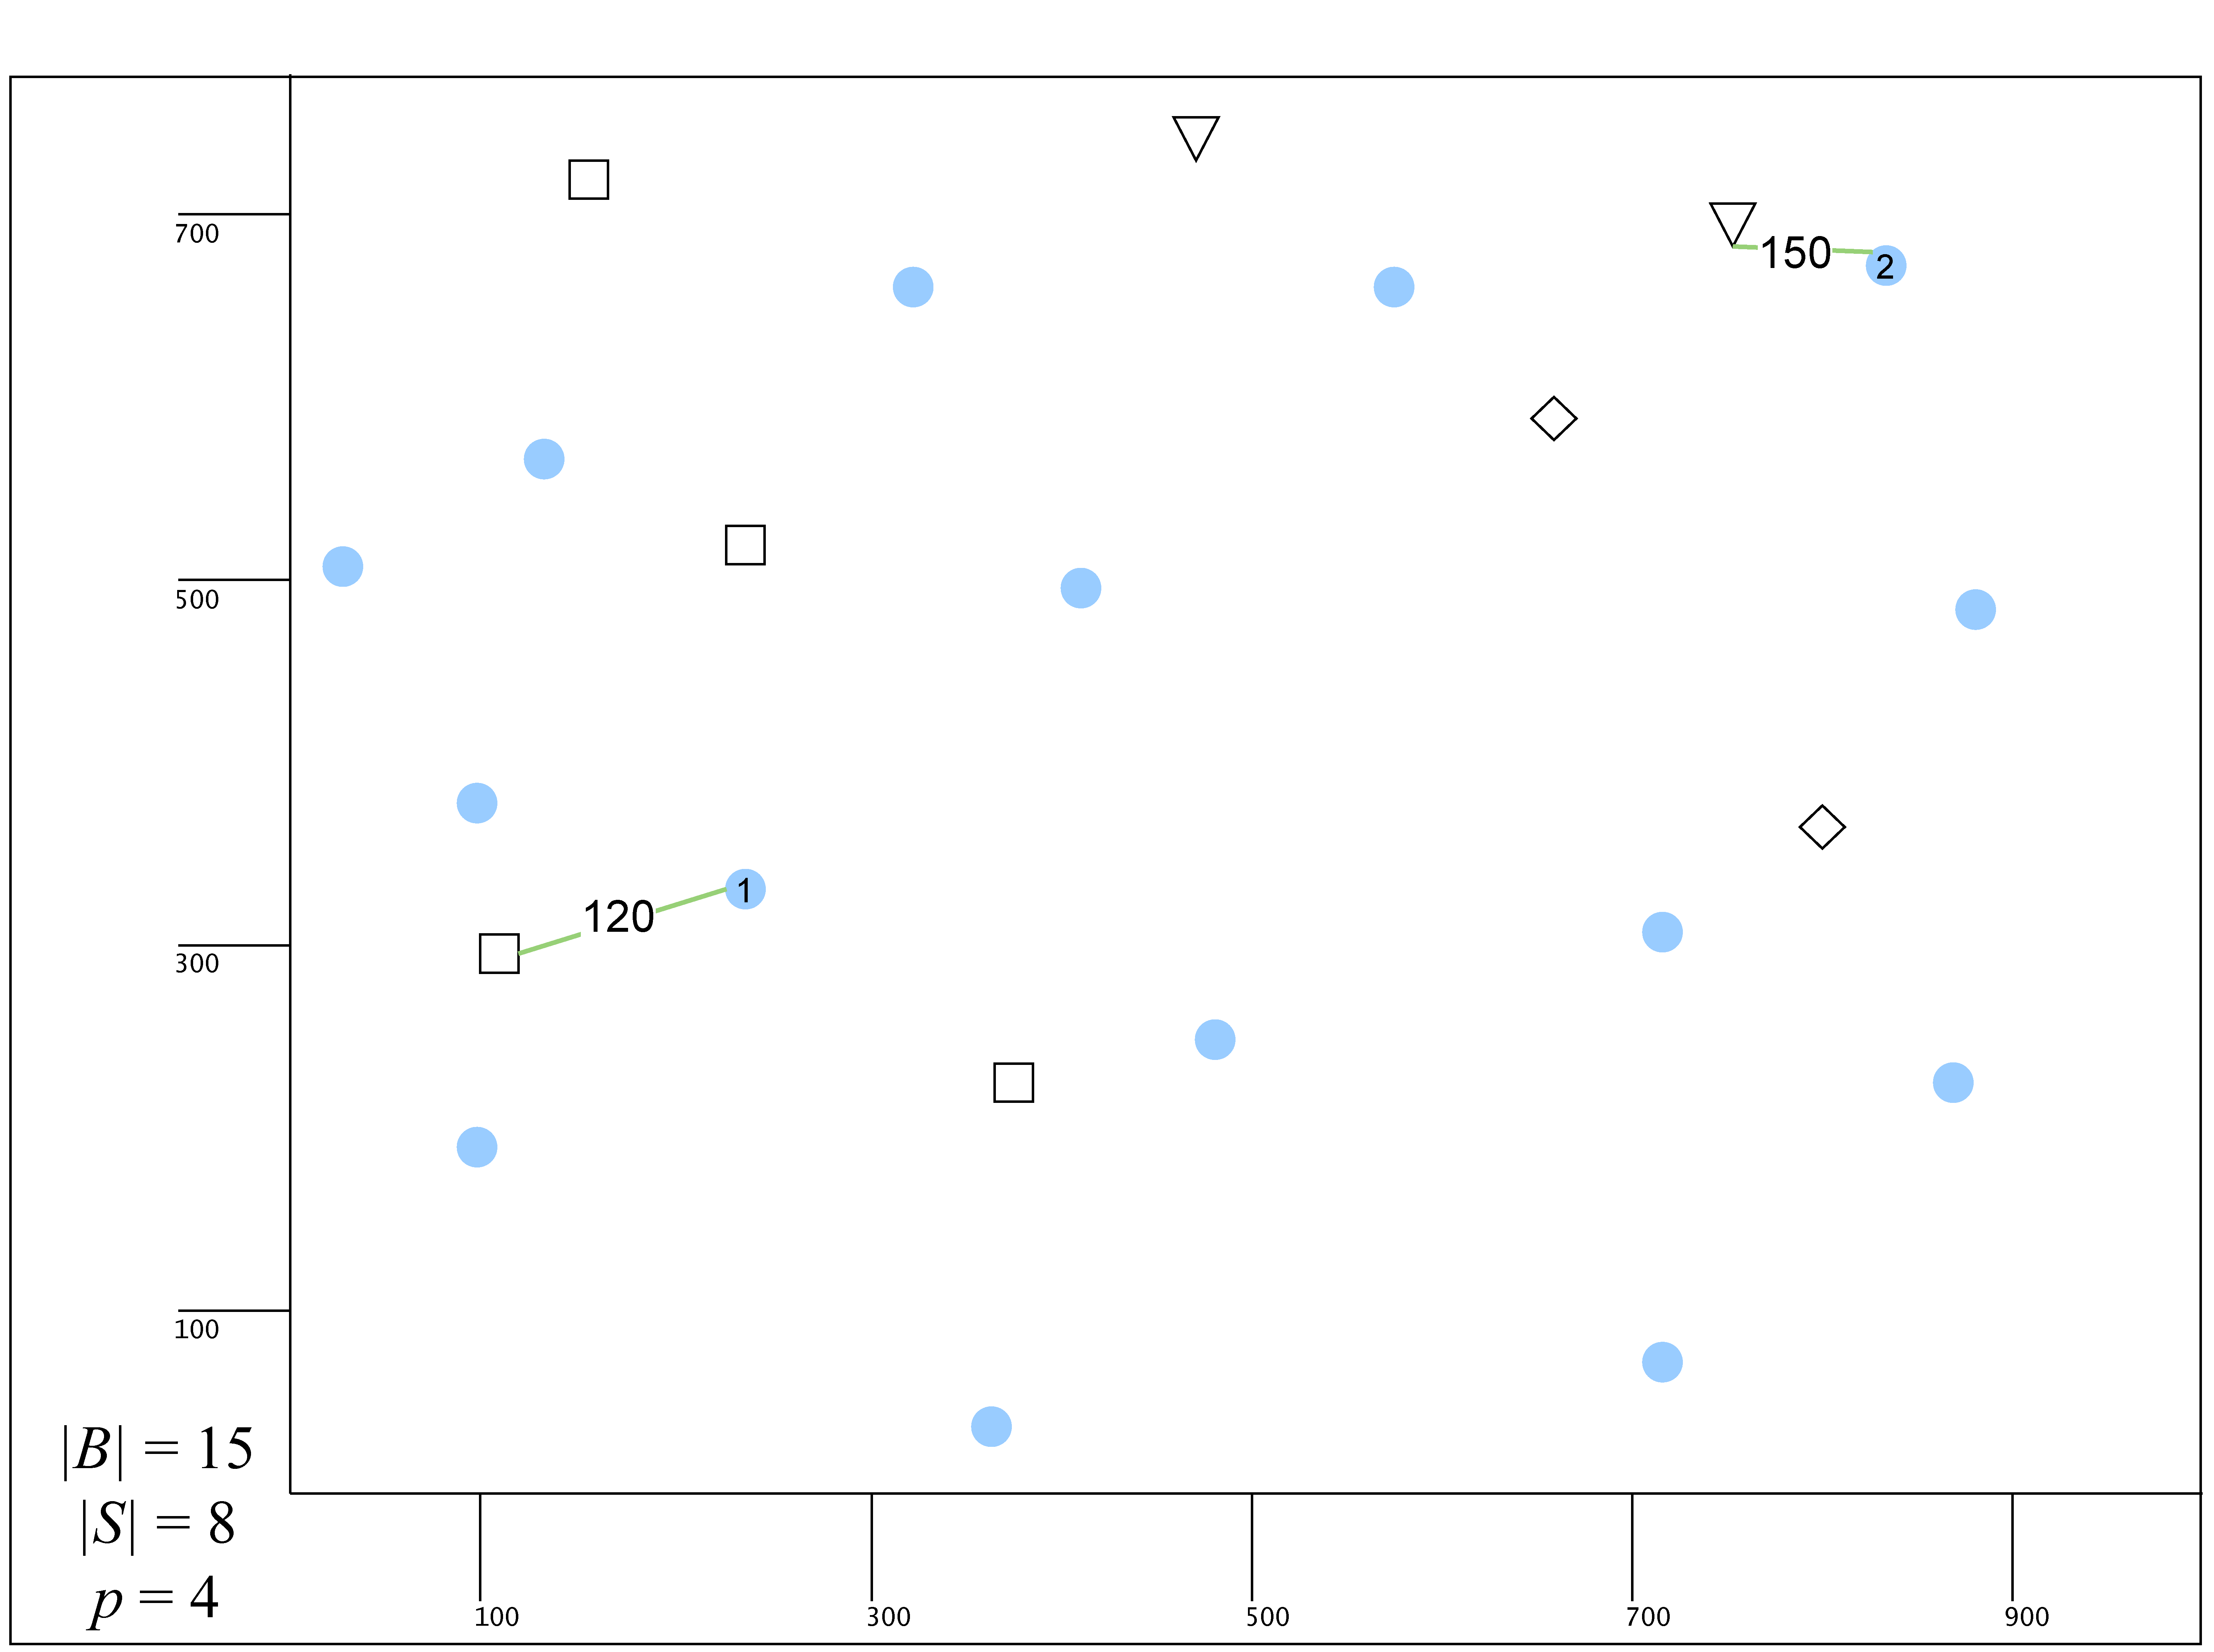
\includegraphics[scale=0.076]{images/opp_1.pdf}
    \end{figure}
\end{frame}

\begin{frame}{Cost of Opportunity}
    \framesubtitle{Explanation}
    Get the furthest possible allocation and compute the cost of opportunity, selecting the largest:
    \begin{figure}
        \centering
        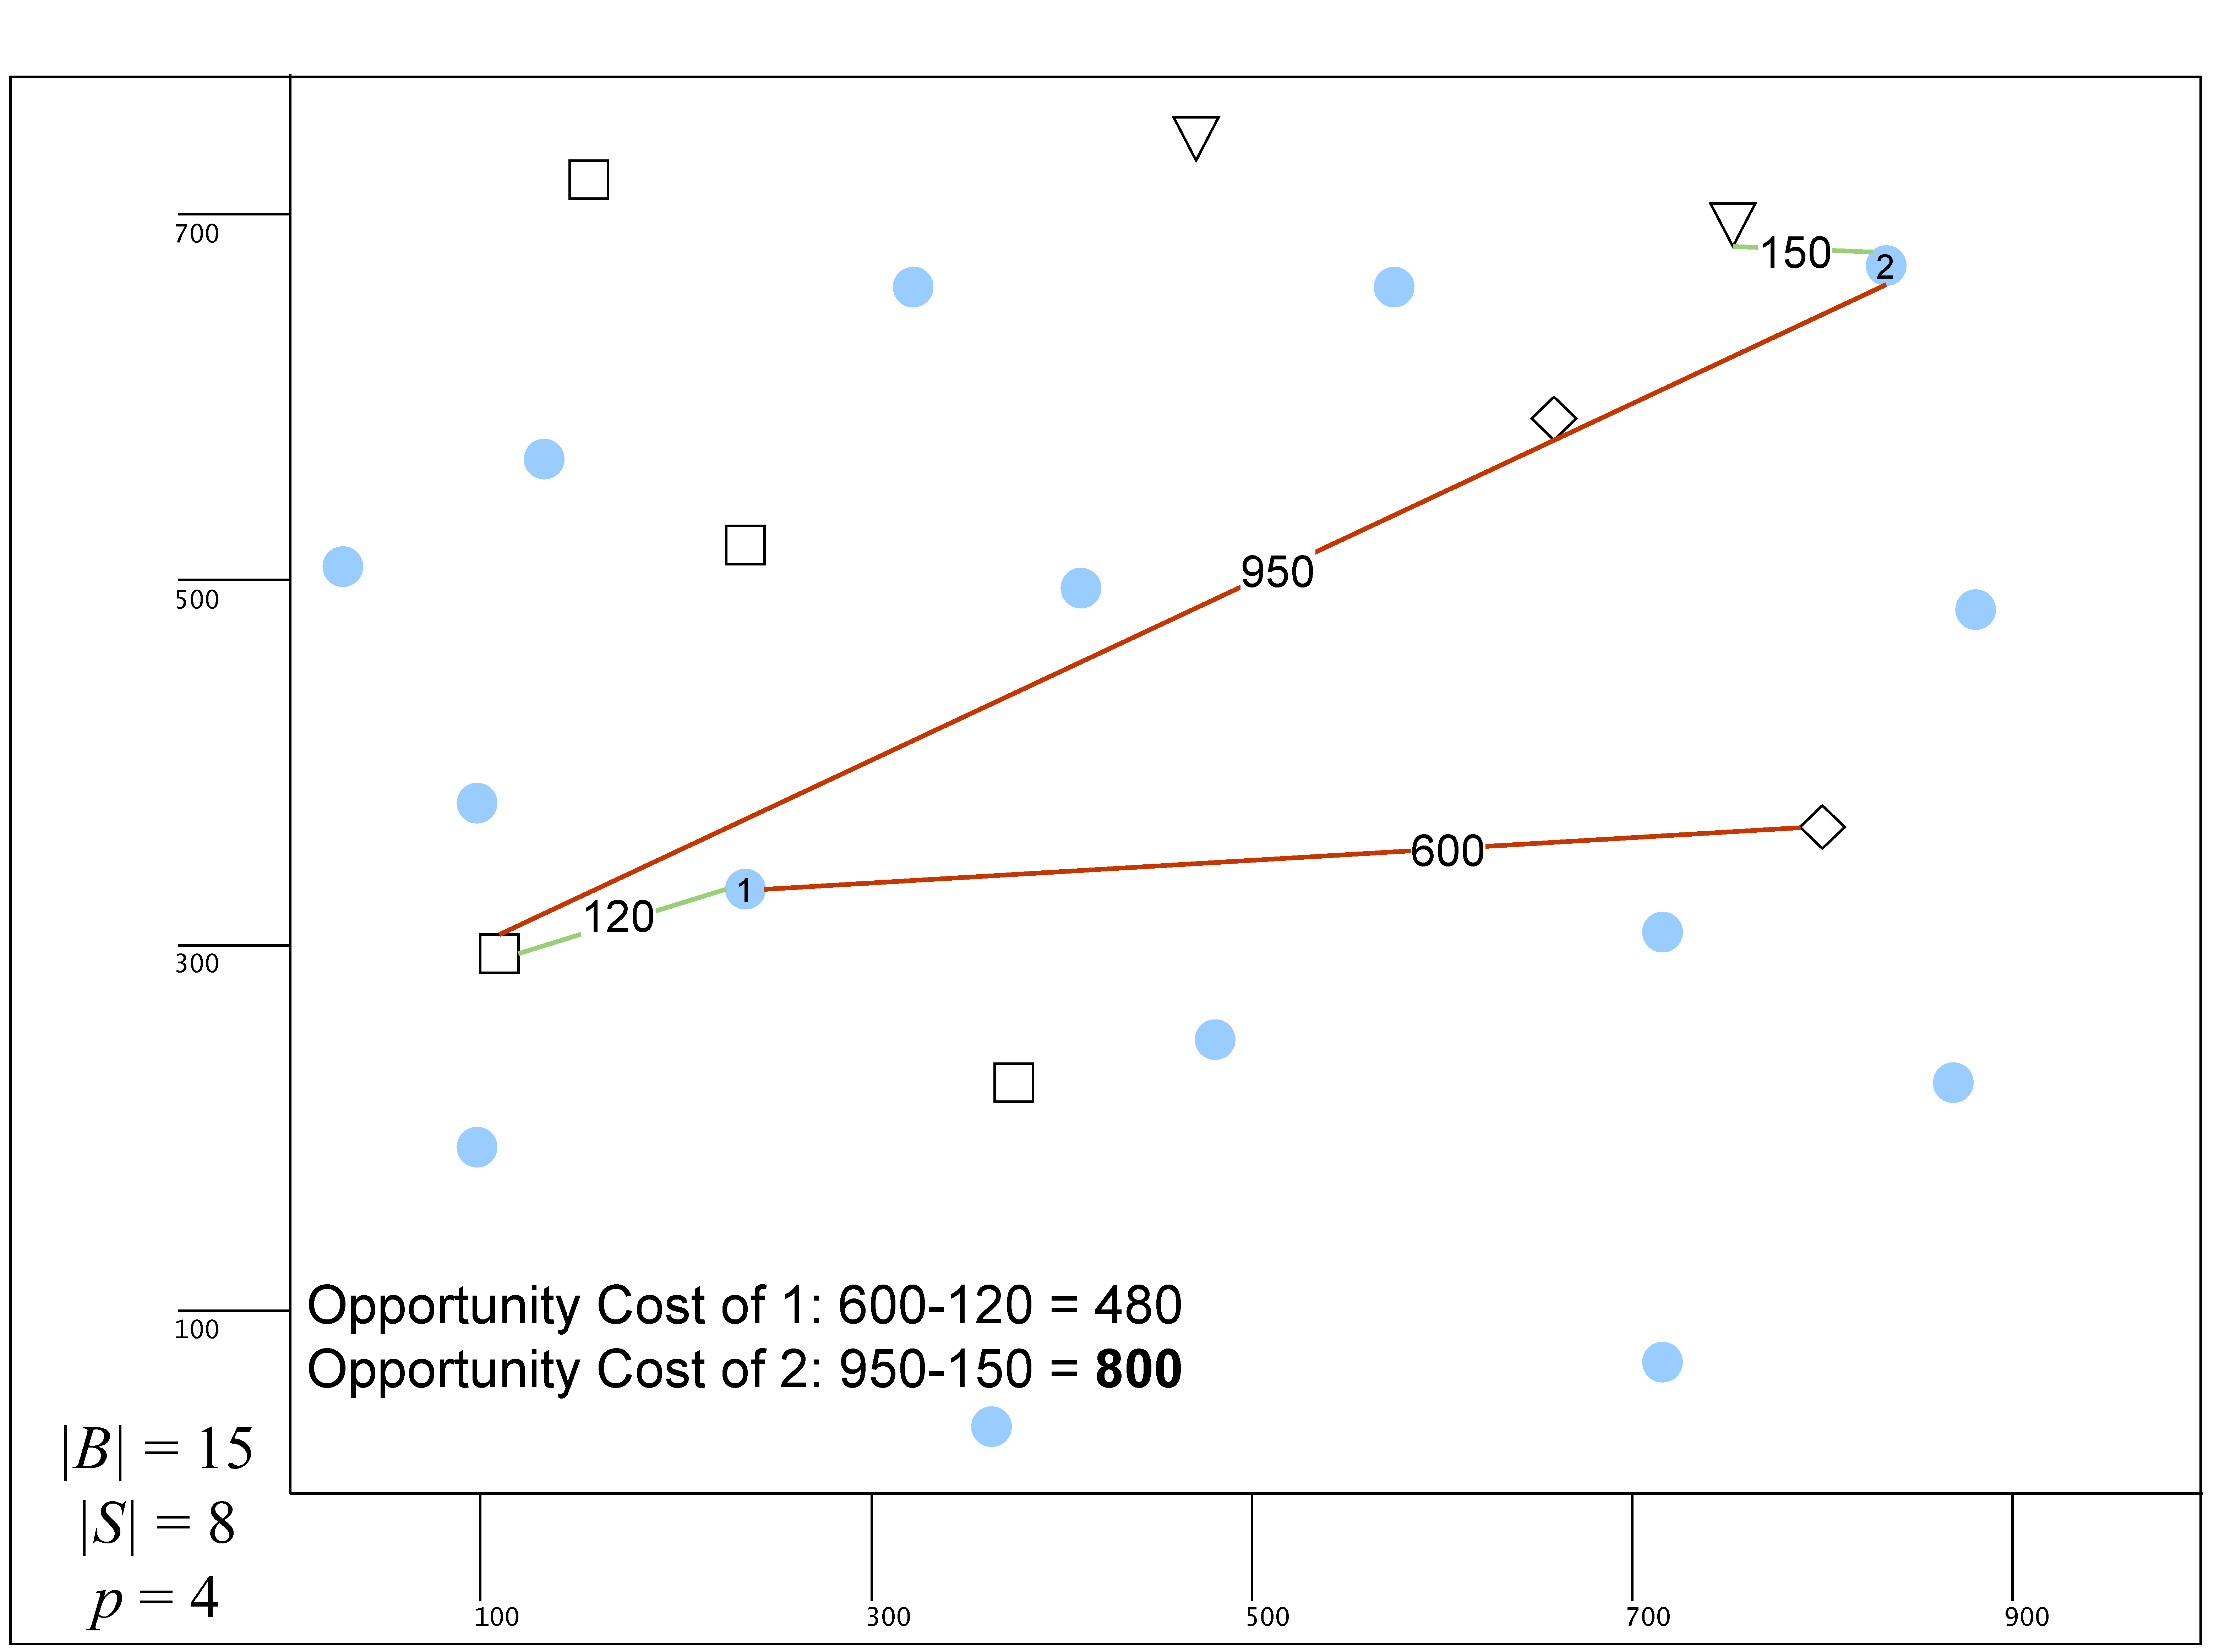
\includegraphics[scale=0.076]{images/opp_2.pdf}
    \end{figure}
\end{frame}
\begin{frame}{Cost of Opportunity}
    \framesubtitle{Explanation}
    By calculating the opportunity cost of every BU and selecting first the largest ones, we try to ensure that the BUs that could be most affected by constraints and unusable centers are allocated first. 
    In the first approach, we calculated the costs of all centers for each BU, generating a matrix with the same size as $d$. In the second approach, we only calculate the largest opportunity cost and store it in a priority queue. 
\end{frame}

\begin{frame}{Cost of Opportunity}
    \framesubtitle{Data Structures}
    During testing we found that most of the time the heuristic spent was on memory allocations and copies related to the traversal and updating of the cost of opportunity matrix. The worst case scenario $\mathcal{O}(n)$ for this approach is $\mathcal{O}(B^2*S)$.
    \\
    Instead of recalculating maximums and minimums, we precompute a cost of opportunity priority queue, which automatically sorts the BUs by that metric as well as precalculating a dictionary of nearest assignments for all BUs, with each BU being a key. The worst case scenario $\mathcal{O}(n)$ for this is $\mathcal{O}(B*S)$. 
\end{frame}

\begin{frame}{Cost of Opportunity}
    \framesubtitle{Guaranteeing feasibility}
        During the traversal of the queue, we mark centers as full when their activity measure reaches the lower bound of the activity measures target. In doing so, we guarantee that all the centers are evenly distributed, ensuring the lower bound is met and by consequence the upper bound is never surpassed, as the location phase also generates feasible $Y$ vectors, guaranteeing mostly feasible solutions.
\end{frame}

\begin{frame}{Cost of Opportunity}
    \framesubtitle{Partial evaluation}
    Moreover, if during each allocation we know which specific $i$ and $j$ are being used, we use additional data structures to represent the activity measures, updating just for $i$ and $j$. When checking if the move is feasible, we don't have to compute the feasibility of all the solution, just of the specific center $i$, adding the activity measure values and risk of $j$. This idea is also used in the local search.
\end{frame}

\begin{frame}{Cost of Opportunity}
    \framesubtitle{Pseudocode of Precomputing}
    \scalebox{0.7}{
    \begin{minipage}{1.8\linewidth}
    \begin{algorithmic}[1]
        \STATE Calculate Opportunity Cost, $\quad \forall j \in B$, store in priority queue $pq$
        \STATE Compute and Order the Best Assignments, $\quad \forall j \in B$, store in dictionary $best\_assignments$
        \STATE Initialize \textit{assigned\_clients} as an empty set
        \STATE Initialize \textit{full\_centers} as an empty set
        \STATE Initalize \textit{values\_matrix, risk\_vec} as auxiliary data structures for feasibility state
    \end{algorithmic}
    \end{minipage}
    }
\end{frame}

\begin{frame}{Cost of Opportunity}
    \framesubtitle{Main Loop}
    \scalebox{0.7}{
    \begin{minipage}{1.8\linewidth}
    \begin{algorithmic}[1]
        \STATE Precompute the data structures.
        \WHILE{$pq$ is not empty \AND $\lvert assigned\_clients \rvert < B$}
            \STATE $j$ $\leftarrow$ dequeue $pq$
            \IF{$j$ $\notin$ \textit{assigned\_clients}}
                \FOR{each $i \in$ \textit{best\_assignments}[$j$]}
                    \IF{$i \notin$ \textit{full\_centers} \AND $Y[i] = 1$}
                        \STATE $X[i, j] \gets 1$
                        \STATE Add client to \textit{assigned\_clients}
                        \STATE Update \textit{values\_matrix, risk\_vec} with $i, j$
                        \IF{$\sum_{j\in B}X_{ij}v_j^m, \forall i \in S \ge Y_i\mu_i(1-t^m)$}
                            \STATE Add $i$ to \textit{full\_centers}
                            \STATE Break
                        \ENDIF
                        
                    \ENDIF
                \ENDFOR
            \ENDIF
        \ENDWHILE
    \end{algorithmic}
    \end{minipage}
    }
\end{frame}

\begin{frame}{Local search}
    \framesubtitle{Repairing unfeasible solutions}
    \scriptsize The opportunity cost matrix approach didn't guarantee feasibility, thus repair moves for the local search are defined as follows.
        \begin{block}{Add($i$)}
        \centering
         \footnotesize If a center $i$ is violating lower bound constraints, then BUs must be assigned to it, until the bound is met. These BUs are removed from other centers, taking into account that in the process, those previou centers don't become unfeasible.
    \end{block}
    \begin{block}{Remove($i$)}
        \centering \footnotesize
        If a center $i$ is violating upper bound constraints, then BUs from this center must be reallocated to other centers, until the bound is met. Again, in this process we must check that those new allocations don't generate unfeasible centers.
    \end{block}
    Instead of performing a normal local search, by guiding it with "Add" or "Remove" sets of the centers, the computation is made faster.
\end{frame}

\begin{frame}{Local search}
    \framesubtitle{Improving solutions}
    \scriptsize Once a solution is feasible, the following local search moves are performed following a Variable Neighborhood Descent approach.
        \begin{block}{Allocate\_Other($i, j$)}
        \centering
         \footnotesize Move BU $j$ from the current allocated center $i$ to any other center $\tilde{i} \in S, \tilde{i} \ne i$
    \end{block}
    \begin{block}{Interchange($i, j, \tilde{i}, \tilde{j}$)}
        \centering \footnotesize
        Interchange the allocations of BUs $j$ and $\tilde{j}$, assigning $j$ to $\tilde{i}$ and $\tilde{j}$ to $i$.
    \end{block}
    \begin{block}{Deactivate($i, \tilde{i}$)}
        \centering \footnotesize
        Mark a currently used center $i$ as closed, open a center $\tilde{i}$ which was previously unusable, assign clients to the the newly opened $\tilde{i}$ center until lower bounds are met, allocate the orphaned BUs served by $i$ to their best possible assignments across all centers.
    \end{block}
\end{frame}

\section{Empirical work}

\begin{frame}{Experiments layout}
    \framesubtitle{Computational results}
    The heuristics were coded in Julia 1.9.0. \\
    The source code is released as FOSS and it can be found in the following repository: \url{https://github.com/eduardosalaz/tesis}.\\
    The computing platform has an Intel Core i5-9300 2.5 GHz processor with 16 GB of RAM under Windows 10.\\
    For the experiments, instances were generated with BUs and Centers' coordinates located randomly between 5 and 10,000 along with the center types, risk and activity measures.
\end{frame}

\begin{frame}{Exact Solver Comparison}
    Part of the methodology of the experiments involved programming the mathematical model in order to feed it to an exact solver, in this case Gurobi 9.5.2 to provide a bound to compare the objective function value of the heuristics, with a cutoff time of 1800 seconds. \textbf{Gurobi did found one optimal solution for Dataset 1, for all of the others instances it did not reach the optimal value in the cutoff time}.
\end{frame}

\begin{frame}{Constructive algorithms comparison}
    \framesubtitle{Computational results}

    \begin{block}{Data set}
        \begin{description}
            \item[Size 1] 20 instances with 625 BUs, 62 centers and 32 to be located.
            \item[Size 2] 20 instances with 1250 BUs, 155 centers and 62 to be located.
        \end{description}
    \end{block}
\end{frame}

\begin{frame}{Constructive algorithms comparison}
    \framesubtitle{Computational results}
\begin{table}
    \centering
    \scalebox{0.5}{
        \begin{tabular}{|c|c|c|c|c|c|c|c|c|c|c|}
    \hline
    \multirow{2}{*}{Dataset} & \multirow{2}{*}{Location} & \multicolumn{2}{c|}{\%Feasible} & \multicolumn{2}{c|}{Time allocation} & \multirow{2}{*}{Time location} & \multicolumn{2}{c|}{Total Time} & \multicolumn{2}{c|}{\%GapGurobi} \\
    \cline{3-4} \cline{5-6} \cline{8-9} \cline{10-11}
     &  & Matrix & Queue & Matrix & Queue & & Matrix & Queue & Matrix & Queue \\
    \hline
\multirow{2}{*}{1} & P-disp & 0 & 0 & 387.10 ms & \textbf{1.60 ms} & 2.40 ms & 1842.70 ms & \textbf{443.35 ms} & 41.82 & 51.87 \\
    \cline{2-11}
     & Relax & 0 & 0 & 445.80 ms & 28.55 ms & 1 s & 3162.15 ms & 1415.20 ms & 48.32 & 54.91  \\
    \hline
    \multirow{2}{*}{2} & P-disp & 0 & \textbf{90} & 3287 ms & \textbf{22 ms} & 5.80 ms & 11 s & \textbf{24 ms} & 70.12 & 88.91 \\
    \cline{2-11}
     & Relax & 0 & 85 & 3283 ms & 33.52 ms & 7 s & 23.73 s & 7 s & 74.62 & 79.52  \\
    \hline
    \end{tabular}
    }
    \caption{Constructive Heuristics Comparison of Averages.}
    \label{:comp}
\end{table}
    Total Time column includes Time Spent in the Repair Solution Phase. Not noted in table, but for Dataset 1, solutions constructed with the queue allocation method violate on average 5 constraints, whereas matrix method violates 46 constraints on average.
    \\
    Based on these results, it was decided to use the $p$-dispersion heuristic as the Location Phase and the Opportunity Cost Queue as the Allocation Phase for the Constructive Phase of the GRASP Procedure.
\end{frame}

\begin{frame}{Local Search algorithms comparison}
    \framesubtitle{Computational results}
    \begin{table}
        \centering
        \scalebox{0.7}{
        \begin{tabular}{|c|c|c|c|c|}
            \hline
            Dataset & Strategy & \% Relative Improvement & \%Gap to Gurobi & Time Spent \\
            \hline
            \multirow{2}{*}{1} & BF & 95.6 & 9.95 & 366.47 ms \\
            \cline{2-5}
             & FF & 67.12 & 12.33 &  \textbf{275.32 ms} \\
            \hline
            \multirow{2}{*}{2} & BF & 83.45 & 9.85 &  3036.79 ms\\
            \cline{2-5}
             & FF & 71.23 &  10.85 & \textbf{1880.61 ms} \\
            \hline
        \end{tabular}
        }
        \caption{Local Search Heuristics Comparison of Averages.}
        \label{tab:ls_improv_exp}
    \end{table}
   Due to the nature of the VND, tracking each individual move's contribution and runtime proved difficult, therefore we present the whole local search results. As we see, the FF strategy is faster with acceptable gaps to the best value found by Gurobi. Early tests without the Deactivate move presented much worse results, leading us to conclude that this move despite being the most computationally complex is the one that improves the most.
\end{frame}

\begin{frame}{Heuristics results with larger sized instances}
    \framesubtitle{Computational results}
    \begin{itemize}
        \item $p$-dispersion as \textbf{location component}, 
        \item opportunity cost queue as \textbf{allocation component}
        \item First Found strategy for the \textbf{Local Search}
    \end{itemize}
    \begin{block}{Data set}
        \begin{description}
            \item[Size 3] 10 instances with 2500 BUs, 325 centers and 125 to be located. Gurobi was configured with a cut-off time of 2 hours.
        \end{description}
    \end{block}
    On average, the constructive heuristic ran for \textbf{110.9 ms}, the local search heuristic for \textbf{14.77 s}, with a total time of \textbf{14.87 s}. The gap to the best solution found by Gurobi is on average \textbf{9.76\%}, whilst being \textbf{483.2 times (48,320\%) faster} than the solver.
\end{frame}

\begin{frame}{GRASP}

Instead of choosing greedily the centers and BUs that provide the best minimal distance to the solution, we also include those that are within an $\alpha$ fraction of the best distance and store them in a Restricted Candidate List, picking at random from this RCL, allowing for a mix of greediness and randomness, providing a unique solution for each iteration. One advantage of GRASP is that it fits a parallel model of computing.
\\
In this case, we define an $\alpha_l$ for the location component and an $\alpha_a$ for the allocation component. 
\end{frame}

\begin{frame}{GRASP: Multi-threaded performance}
    As stated before, GRASP can be parallelized. We ran a basic GRASP setup with $\alpha_a=0.3, \alpha_l=0.3$ and \textit{max\_iters} = 90 and tested for the optimal number of threads to run the GRASP with. Hypothesis testing of ANOVA was performed to check if the number of threads had an effect on the objective function value, with the results showing that there's no significant impact (p-value: 0.9989)
    \begin{figure}
        \centering
        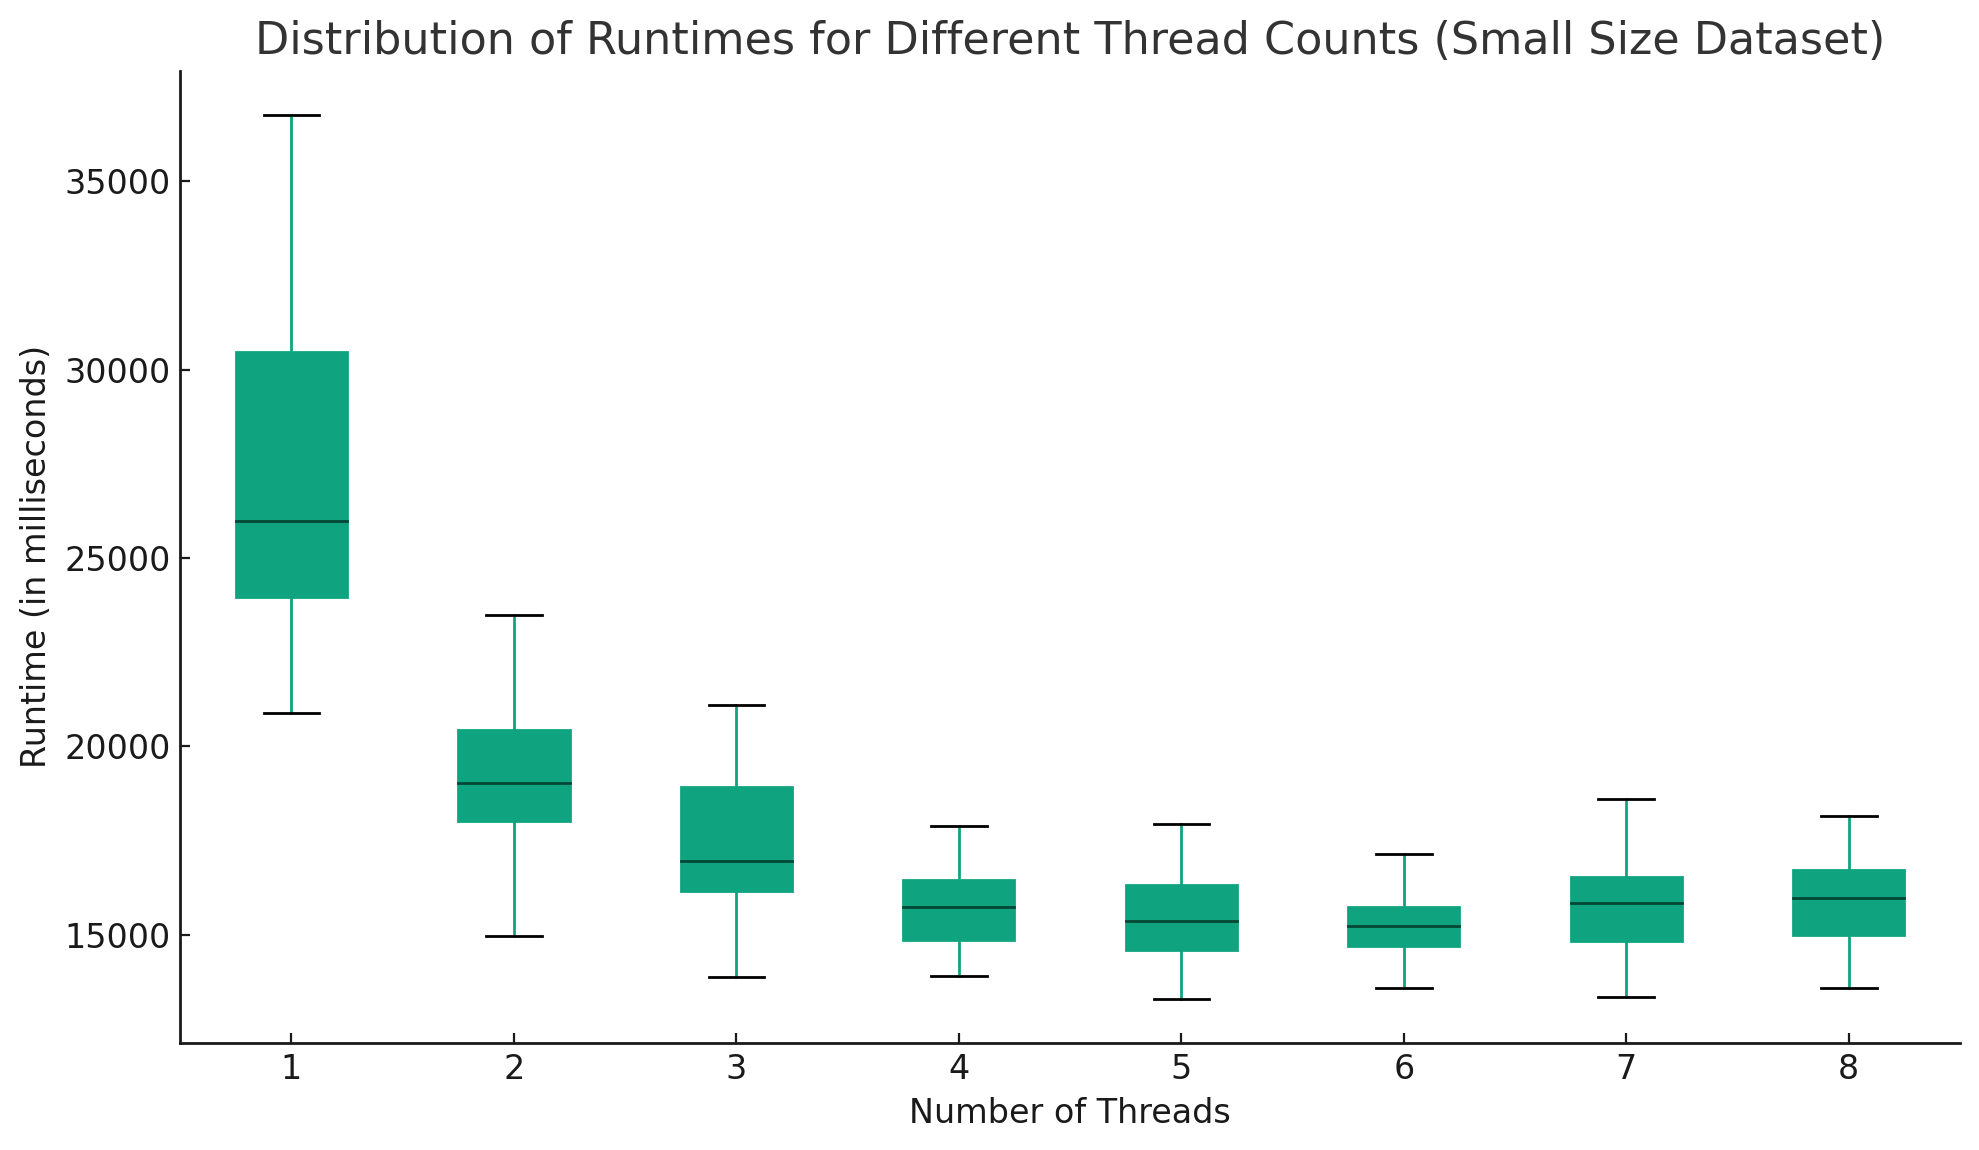
\includegraphics[scale=0.31]{boxplot_small.png}
    \end{figure}
\end{frame}

\begin{frame}{GRASP: Multi-threaded performance}
Additional Hypothesis testing (Paired t-tests) was performed as well to determine the optimal number of threads, but visually one can infer that it is 4 when taking into account both datasets. 
        \begin{figure}
        \centering
        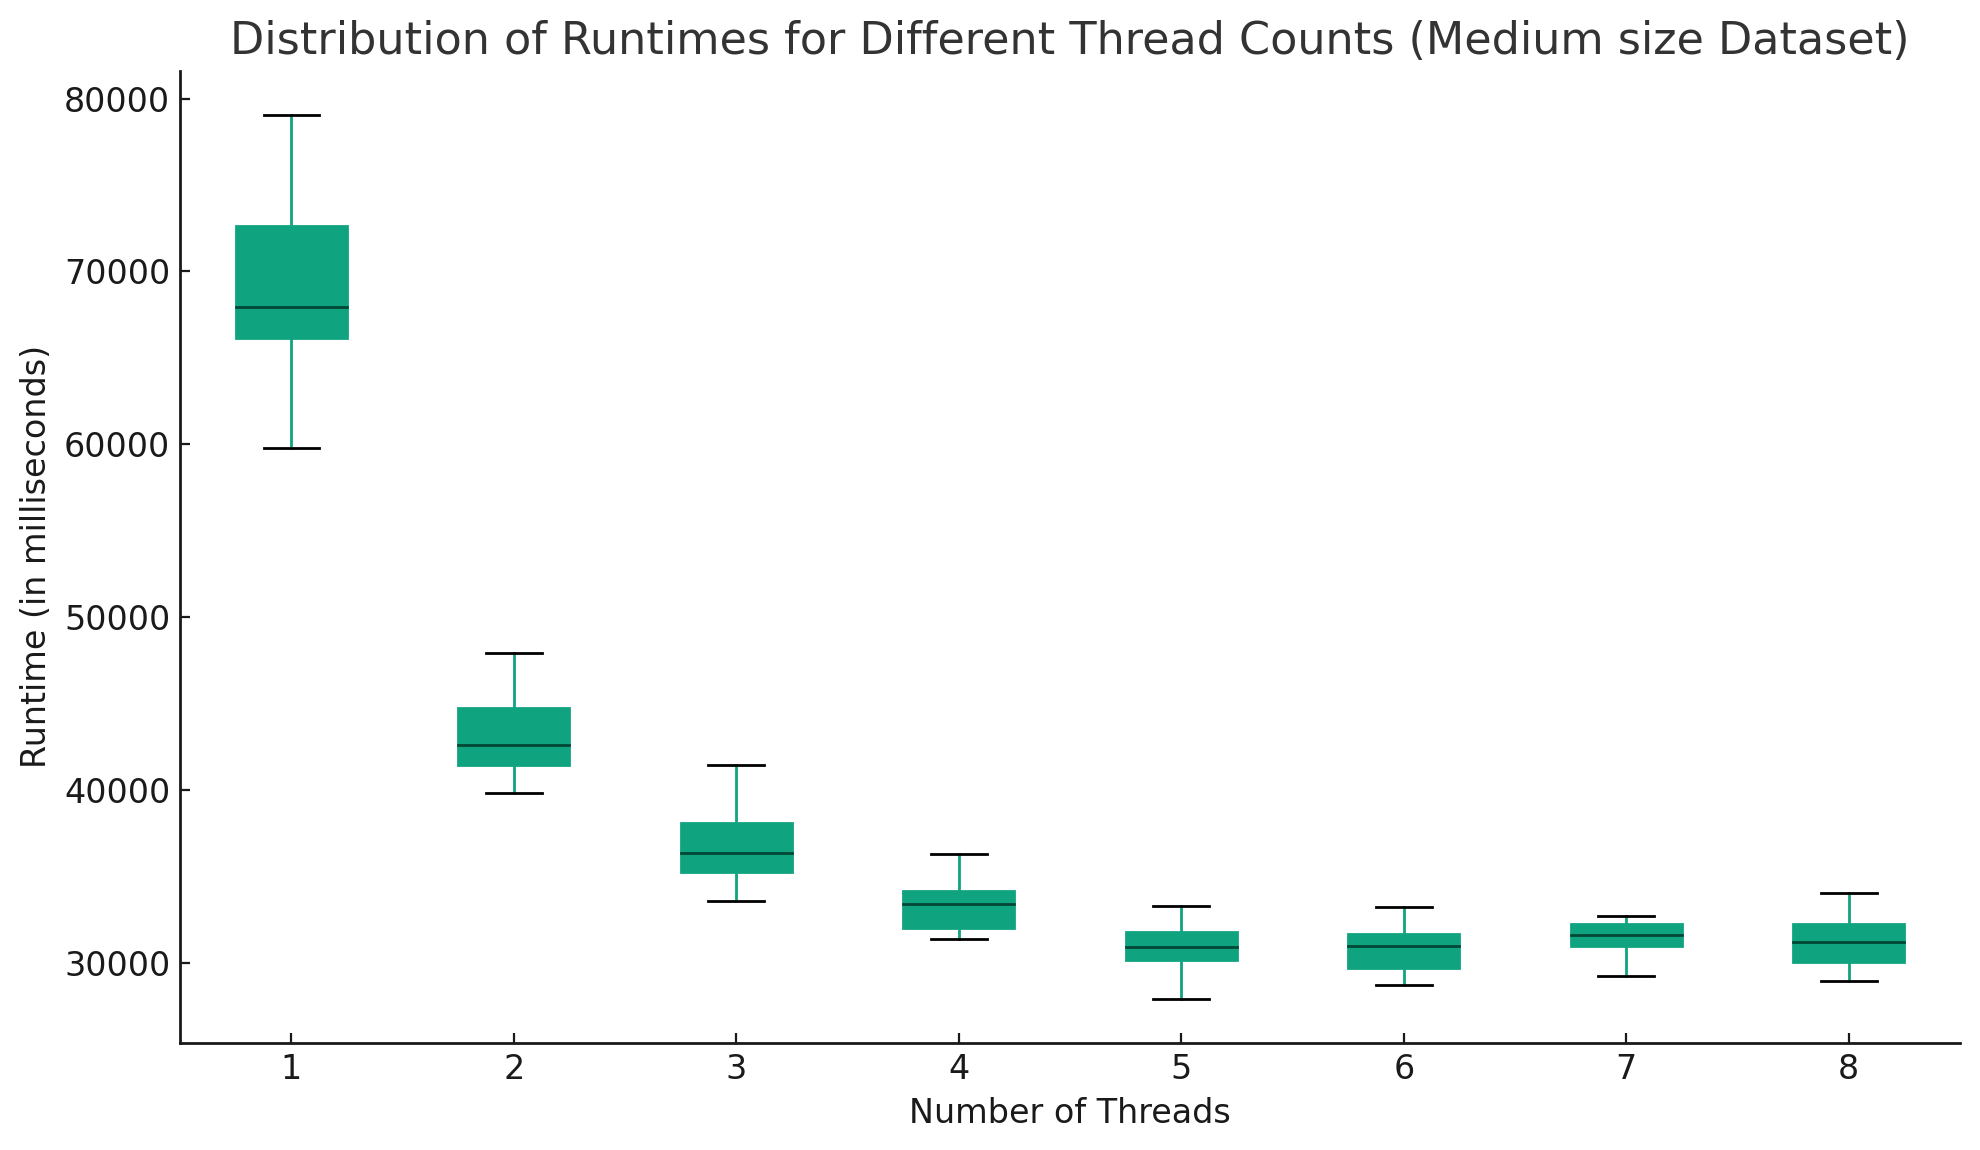
\includegraphics[scale=0.4]{boxplot_medium.png}
    \end{figure}
\end{frame}

\begin{frame}{GRASP: Calibration of parameters}
As stated before, we have 3 parameters to calibrate: $\alpha_l, \alpha_a$ and number of iterations. We tested the following combinations, for a subset of solutions from Datasets 1 and 2 for a total of 125 configurations.
    \begin{itemize}
        \item $\alpha_l \in \{0.1, 0.3, 0.5, 0.7, 0.9\}$
        \item $\alpha_a \in \{0.1, 0.3, 0.5, 0.7, 0.9\}$
        \item \textit{max\_iters} $\in \{10, 30, 50, 70, 90\}$
    \end{itemize}
\end{frame}

\begin{frame}{GRASP: Calibration of parameters}
Factorial ANOVA and One Way ANOVA showed that $\alpha_l, \alpha_a$ had really no effect on neither the objective function nor the runtime and that there were no interaction effects between the parameters. \textit{max\_iters} did had an impact on both runtime and objective function value. Thus, we picked the $\alpha_l, \alpha_a$ that had the best means in runtime, which were $\alpha_l = 0.1, \alpha_a = 0.3$.
\\Increasing the number of iterations from 10 to 90 led to an improvement of approximately 1.541\% in the objective function value. However, this improvement came with a substantial increase in runtime, approximately 717.689\%, thus we settled for 70 iters.
\\
\medskip
\scriptsize The table is not shown as it would be too large.
\end{frame}

\begin{frame}{GRASP: Calibration of parameters}
\begin{figure}
        \centering
        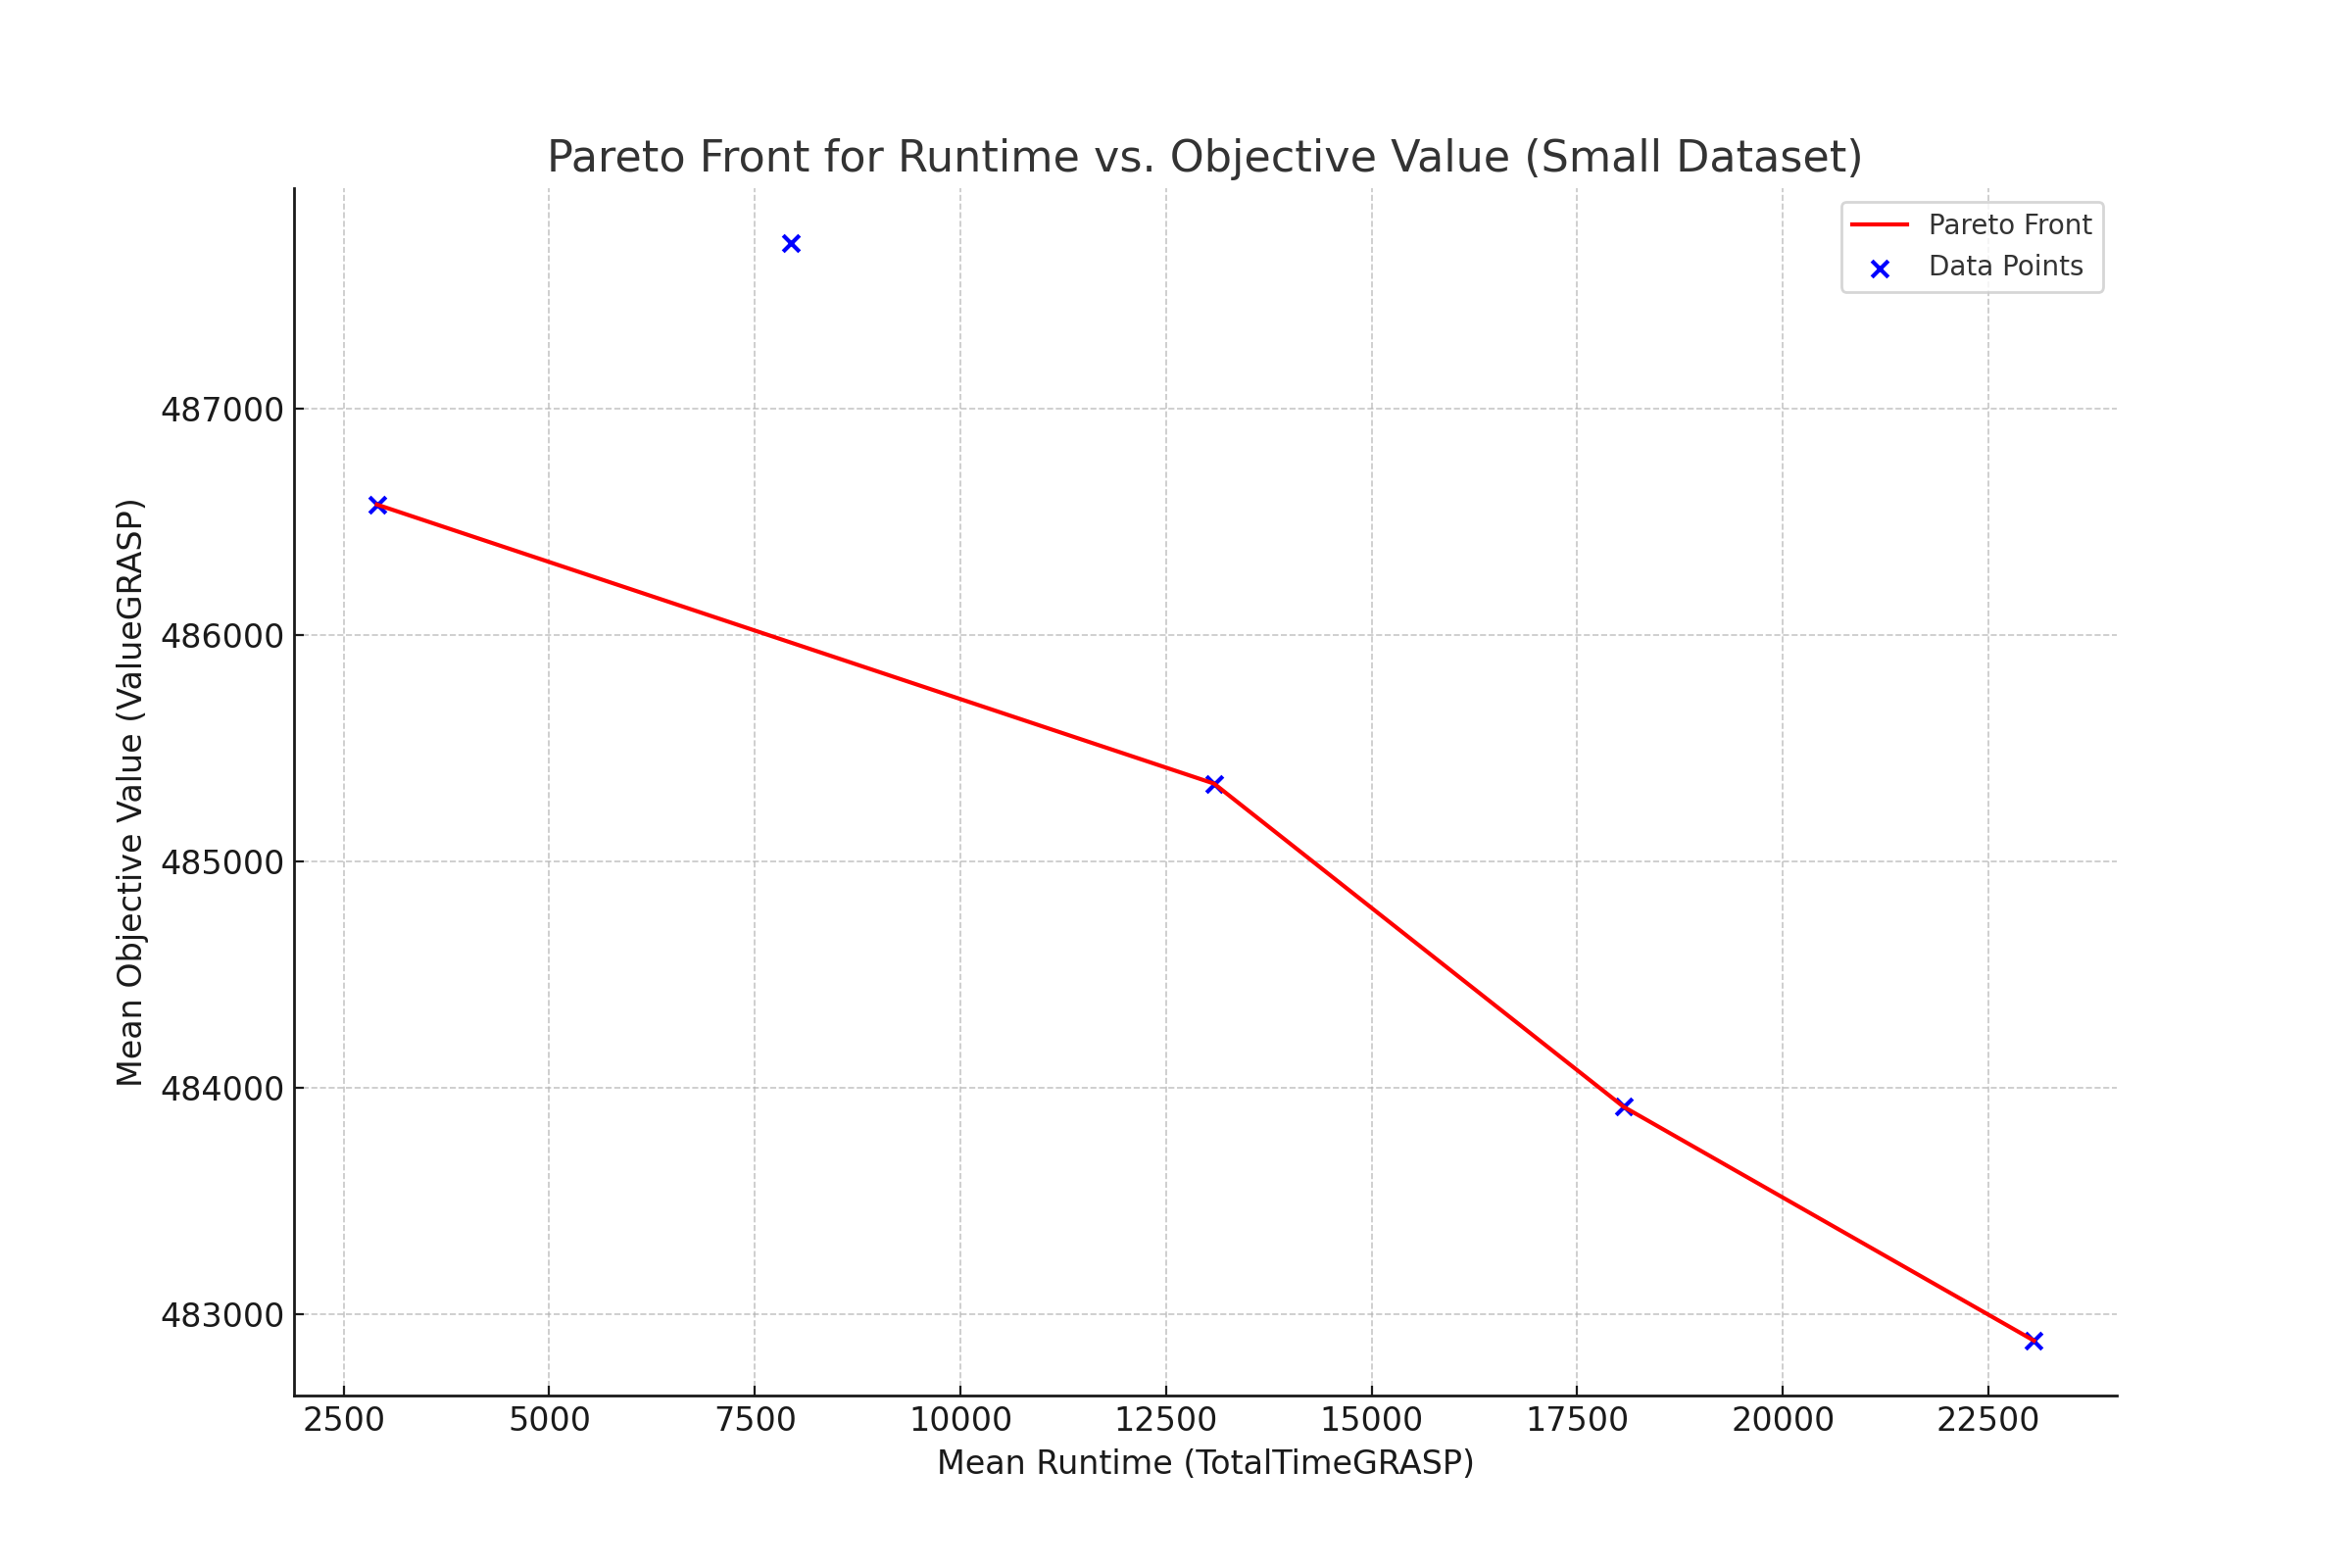
\includegraphics[scale=0.3]{pareto_front_small.png}
    \end{figure}
\end{frame}
\begin{frame}{GRASP: Calibration of parameters}
\begin{figure}
        \centering
        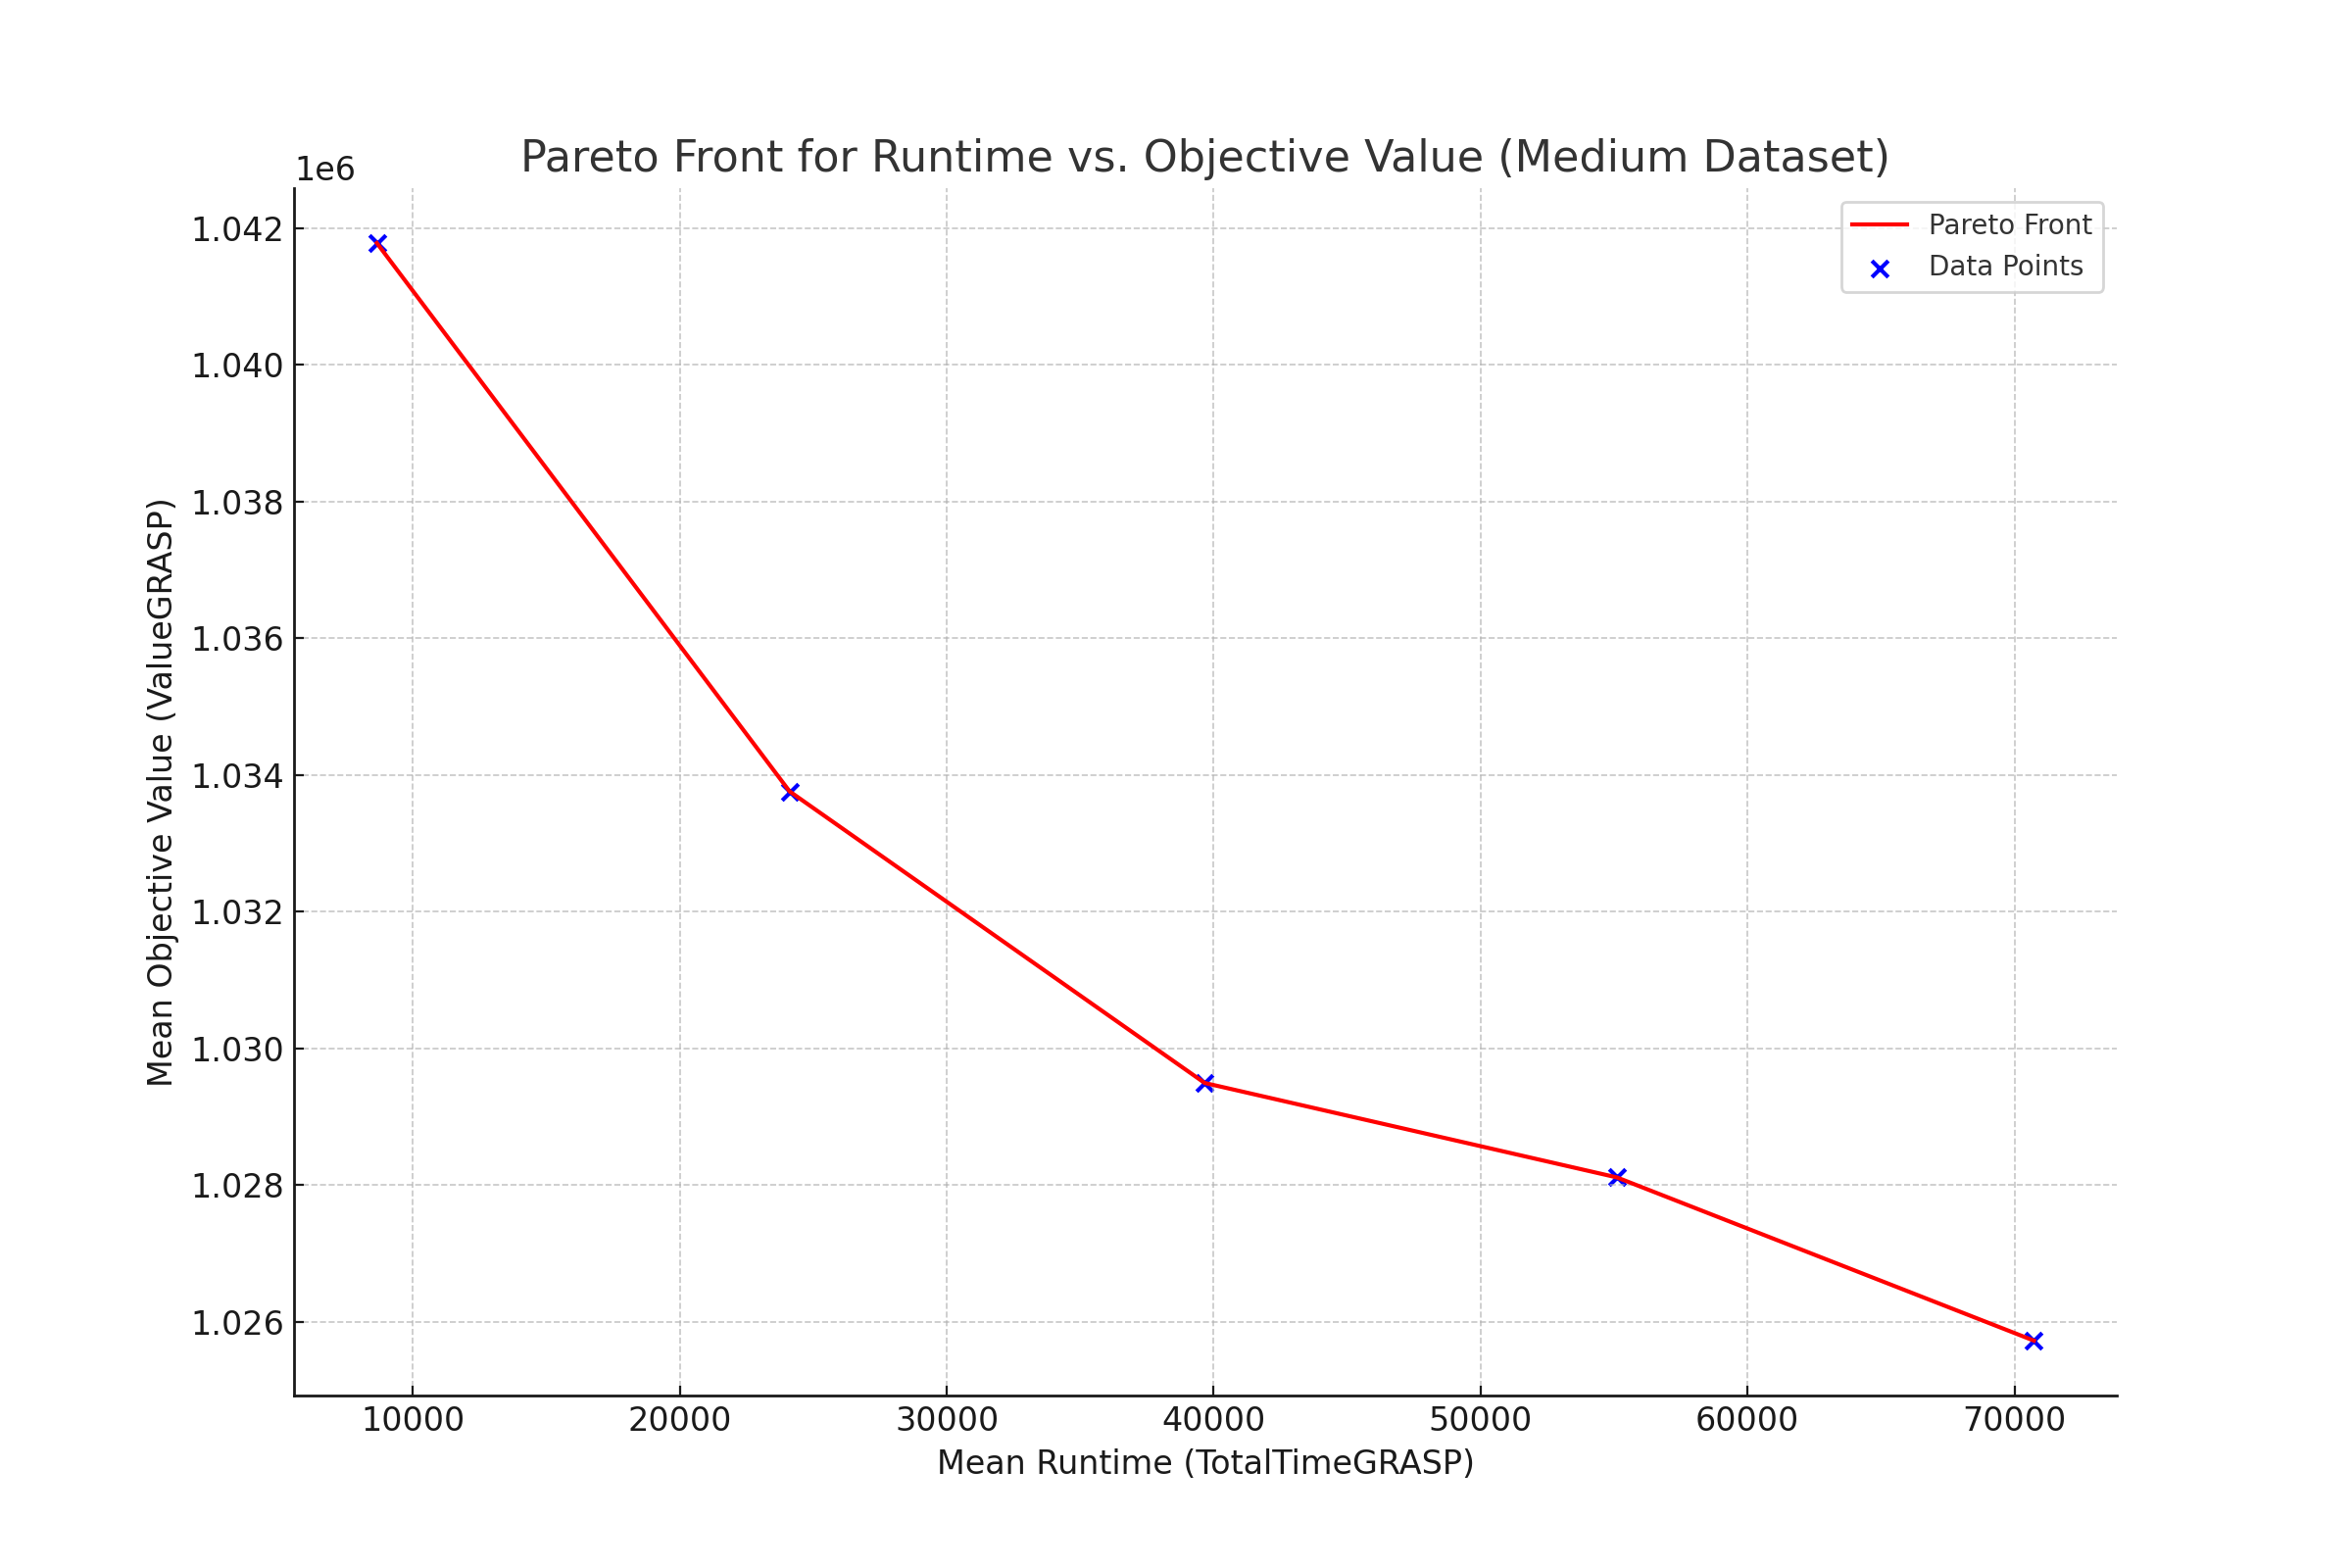
\includegraphics[scale=0.3]{pareto_front_medium.png}
    \end{figure}
\end{frame}

\begin{frame}{GRASP Results}
    \begin{table}[h]
    \centering
    \begin{tabular}{|c|c|c|c|}
        \hline
        \textbf{Dataset} & \textbf{Time GRASP} & \textbf{Time Gurobi} & \textbf{\%Gap to Gurobi} \\
        \hline
        1 & 17.05 s & 1800 s & 2.88 \\
        \hline
        2 & 62 s & 1800 s & 5.23 \\
        \hline
        3 & 160 s & 7200 s & 7.91 \\
        \hline
    \end{tabular}
    \caption{Comparison of Average values of Fine-tuned GRASP with 4 threads vs Gurobi}
    \label{tab:comparison}
\end{table}

\end{frame}

\section{Wrap-up}

\begin{frame}{Wrap-up}
    \small Conclusions
    \scriptsize
    \begin{itemize}
        \item Using a $p$-dispersion heuristic as the location heuristic of the problem and the cost of opportunity assignment priority que as allocation heuristic, we get the most feasible and fastest solutions from the constructive heuristic, with the FF strategy for the local search providing a slight edge over the BF on runtime in the local search.
        \item On fine-tuning stage of GRASP, it was observed that a value of \textit{max\_iters}= 70, $\alpha_l = 0.1, \alpha_a = 0.3$ provided the best compromise between runtime and objective function value.
        \item GRASP provides solutions that are marginally worse than the ones provided by Gurobi while being several orders of magnitude faster. In fact, in the Dataset 1, GRASP reached solutions better than the ones found by Gurobi.
    \end{itemize}
    \small Future work
    \scriptsize
    \begin{itemize}
        \item Model the risk as an uncertainty measure.
        \item Introduce contiguity constraints.
        \item Explore hibridization strategies with the exact formulation.
        \item Explore other strategies (TS, ILS, IGLS, VNS, SS).
    \end{itemize}
\end{frame}

\begin{frame}{Acknowledgments}
    \begin{itemize}
        \item Thank you very much for your attention!
        \item Feedback is welcome :)
        \item Email: eduardosalaz@outlook.com
        \item GitHub: \url{https://github.com/eduardosalaz}
    \end{itemize}
    
    \begin{figure}
        \centering
        
\includegraphics[scale=0.2]{uanl-logo}
        
\includegraphics[scale=0.15]{fime-logo}
    \end{figure}
\end{frame}

\begin{frame}{References}
\scalebox{0.8}{
\begin{minipage}{1.1\linewidth}
\printbibliography
\end{minipage}
}

\end{frame}
\end{document}